%==============================================================================
%  An Integrated, Explainable, and Auditable Pipeline for Personal Financial
%  Risk Assessment and Cryptocurrency Portfolio Recommendation
%
%  LaTeX source (single-column IEEEtran).  This is a faithful format conversion
%  of the Word manuscript "DeFi_AI_Assistant_IEEE_Paper_v2.docx"; no scientific
%  content, numbers, equations, tables, figures, or references were altered.
%
%  To compile (Overleaf: set compiler to pdfLaTeX):
%     pdflatex main
%     bibtex   main
%     pdflatex main
%     pdflatex main
%==============================================================================
\documentclass[conference,onecolumn,letterpaper]{IEEEtran}

% ---- Encoding & fonts -------------------------------------------------------
\usepackage[T1]{fontenc}
\usepackage[utf8]{inputenc}

% ---- Mathematics ------------------------------------------------------------
\usepackage{amsmath}
\usepackage{amssymb}

% ---- Graphics ---------------------------------------------------------------
\usepackage{graphicx}
\graphicspath{{figures/}}

% ---- Tables -----------------------------------------------------------------
\usepackage{booktabs}
\usepackage{array}
\usepackage{tabularx}
% tabularx column variants (wrapping paragraph columns of stretchable width)
\newcolumntype{L}{>{\raggedright\arraybackslash}X}
\newcolumntype{C}{>{\centering\arraybackslash}X}
\newcolumntype{R}{>{\raggedleft\arraybackslash}X}

% ---- Citations (IEEE numeric, range compression) ----------------------------
\usepackage{cite}

% ---- Cross-references / clickable links (load last) -------------------------
\usepackage[hidelinks]{hyperref}

% ---- Capability-matrix markers (Table I) ------------------------------------
\newcommand{\yes}{\checkmark}          % implemented and evaluated
\newcommand{\partialmark}{$\circ$}     % discussed or partially addressed
\newcommand{\nomark}{\textemdash}      % not addressed

\begin{document}

\title{An Integrated, Explainable, and Auditable Pipeline for Personal
Financial Risk Assessment and Cryptocurrency Portfolio Recommendation}

% ---- Author / affiliation block ---------------------------------------------
% NOTE: the personal-identity fields below are placeholders carried over
% verbatim from the source manuscript. Replace the four bracketed items
% before submission.  <-- REQUIRES USER INPUT
\author{%
\IEEEauthorblockN{[Author Name(s) --- REQUIRES USER INPUT]}
\IEEEauthorblockA{%
\textit{Department of Information Sciences}\\
\textit{University of Education, Lahore --- Vehari Campus, Punjab, Pakistan}\\
Roll No(s). [REQUIRES USER INPUT] $\cdot$ Session [REQUIRES USER INPUT]\\
Supervisor: [REQUIRES USER INPUT]}%
}

\maketitle
\pagestyle{plain}          % centered page numbers, as in the source document

% ---- Abstract ---------------------------------------------------------------
\begin{abstract}
Retail financial-technology tools typically treat risk assessment, explanation,
investment allocation, and record-keeping as separate problems, so a user seldom
receives a single recommendation that is at once data-driven, interpretable,
conservative, and independently verifiable. This paper presents a decision-support
pipeline that unifies these concerns end to end. Five raw, user-supplied inputs are
transformed into three interpretable financial ratios; unsupervised K-means
clustering assigns Low, Medium, and High risk proxy labels; a leakage-aware
multilayer perceptron learns to reproduce those labels from the raw inputs alone
under an explicit feature contract; a deterministic guardrail and a most-cautious
reconciliation rule combine the learned, cluster, and rule-based signals so that the
system can only ever escalate risk; an occlusion-based explainer reports per-input
influence; the reconciled band is mapped to a Bitcoin/Ethereum/USDC allocation and
projected over twelve months; and every recommendation is hashed with SHA-256 into a
verifiable audit record. On a synthetic dataset of 3,000 records the classifier
attains 91.0\% accuracy and a 0.881 macro-F1, with stable clusters (adjusted Rand
index 0.868). The evaluation is held to a deliberately honest standard, and three
findings shape its conclusions: the deterministic guardrail---not the learned
model---binds the final decision for most users, escalating 60.6\% to High risk on
cash-flow grounds; the multilayer perceptron is statistically indistinguishable from
logistic regression (McNemar $p = 0.100$); and two of the three clustering features
are arithmetically recoverable from the classifier inputs. The work is therefore best
read as a contribution in systems integration and transparency rather than in
algorithms: a coherent, inspectable pipeline whose safety and auditability hold by
construction, and whose limitations are measured and disclosed rather than hidden.
\end{abstract}

% ---- Index terms ------------------------------------------------------------
\begin{IEEEkeywords}
Explainable artificial intelligence, financial risk assessment, K-means clustering,
multilayer perceptron, label leakage, portfolio allocation, decentralized finance,
blockchain audit trail, decision-support systems.
\end{IEEEkeywords}

% -----------------------------------------------------------------------------
% Lock the reference numbering to the manuscript's [1]-[22] order.
% IEEEtran.bst lists references in order of first citation; declaring them here,
% in order, guarantees ref1->[1], ref2->[2], ... , ref22->[22] regardless of the
% order in which they are first cited in the body.
% -----------------------------------------------------------------------------
\nocite{ref1,ref2,ref3,ref4,ref5,ref6,ref7,ref8,ref9,ref10,ref11,ref12,ref13,ref14,ref15,ref16,ref17,ref18,ref19,ref20,ref21,ref22}

% ---- Body -------------------------------------------------------------------
% =====================  SECTION I  =====================
\section{Introduction}\label{sec:intro}

\subsection{Background and Motivation}\label{subsec:background}
Retail investing and digital finance have put sophisticated financial decisions in
the hands of individuals who rarely have formal training in risk management.
Artificial-intelligence tools now promise to democratize functions once reserved for
professional advisors, from automated portfolio construction to personalized
financial guidance \cite{ref1,ref2,ref8}, and machine learning has become a standard
instrument for financial forecasting and for flagging individuals at financial risk
\cite{ref3,ref7,ref18}. The same automation that makes these tools scalable also
makes them hard to see into: a retail user is routinely asked to trust a single score
with no explanation of how it was reached and no durable record of what was
recommended or why.

Three concerns have moved to the center of this literature. One is explainability: as
neural models enter financial tasks, methods that attribute a decision to its inputs
have become essential to using them responsibly \cite{ref10,ref12,ref21}. A second is
trust and reliance---behavioral studies of AI financial advisors find that disclosing
a system's limitations, rather than presenting it as infallible, produces more
calibrated user reliance \cite{ref11}. The third, verifiability, follows from the
stakes involved: because financial recommendations carry consequences, tamper-evident
audit trails, often built on blockchain-style hashing, let a recommendation be checked
afterward against what was actually issued \cite{ref13,ref16,ref22}. Cryptocurrency
allocation sharpens all three, since the assets are volatile and the
decentralized-finance setting adds liquidation and stablecoin-stability risks
\cite{ref5,ref6}.

\subsection{Problem Statement and Existing Limitations}\label{subsec:problem}
Despite substantial progress on each concern individually, they are almost always
addressed in isolation. Robo-advisory and portfolio systems optimize allocations but
seldom expose an interpretable risk rationale \cite{ref8,ref12}; distress- and
risk-prediction models classify users but stop short of translating a prediction into
an actionable, safety-constrained recommendation \cite{ref18,ref19}; explainability
research develops attribution methods largely in the abstract \cite{ref10,ref21}; and
blockchain-audit research secures records without connecting them to a live decision
process \cite{ref13,ref14,ref15}. A retail user is thus served by a patchwork of
tools, none of which delivers a recommendation that is simultaneously data-driven,
interpretable, conservative under uncertainty, and independently verifiable. A further
and subtler limitation pervades applied financial machine learning: reported
accuracies are frequently inflated by information leakage between how labels are
constructed and what features a model is given, and by evaluation protocols that do
not account for repeated entities \cite{ref4}. Systems are seldom candid about the gap
between a headline metric and the quality of the decision a user ultimately receives.

\subsection{Research Gap}\label{subsec:gap}
The gap this work addresses is therefore integrative and methodological rather than
algorithmic. No single, inspectable system in the reviewed literature carries a user's
raw financial inputs through interpretable feature construction, unsupervised risk
labeling, a leakage-aware classifier, an explicit safety layer, per-decision
explanation, risk-aligned allocation, and a verifiable audit record---while being
explicit about where information leaks, which component actually determines the
outcome, and what the evidence does and does not support. Closing this gap requires not
a new estimator but a coherent architecture with enforceable properties and an honest
evaluation of them.

\subsection{Objectives and Research Questions}\label{subsec:rqs}
The objective of this work is to design, implement, and critically evaluate an
end-to-end pipeline that integrates the five concerns above into a single
decision-support tool, and to hold that tool to a transparent evidential standard.
This objective is refined into six research questions:

\begin{itemize}
\item[\textbf{RQ1.}] Can a user's financial risk be assessed from a small set of raw,
  deployable inputs while the ratios used to construct the risk labels are withheld
  from the classifier, so that leakage can be reasoned about explicitly?
\item[\textbf{RQ2.}] Do unsupervised clusters over interpretable financial ratios
  correspond to coherent, monotonically ordered Low/Medium/High risk bands suitable as
  proxy labels?
\item[\textbf{RQ3.}] Can a supervised classifier reproduce those proxy labels from the
  raw inputs alone with useful accuracy, and is a neural model warranted over simpler
  baselines?
\item[\textbf{RQ4.}] How can a learned signal, an unsupervised signal, and a
  deterministic rule-based signal be reconciled so that the system's failure mode is to
  over-warn rather than under-warn?
\item[\textbf{RQ5.}] Can a single explanation strategy provide per-decision,
  input-level attributions across different model types without retraining?
\item[\textbf{RQ6.}] Can the reconciled risk band be mapped to a risk-aligned
  cryptocurrency allocation and logged as a tamper-evident, independently verifiable
  record?
\end{itemize}

\subsection{Contributions}\label{subsec:contributions}
Against these questions, the paper makes the following contributions:

\begin{itemize}
\item[\textbf{C1)}] An integrated, end-to-end pipeline that unifies feature
  engineering, unsupervised proxy labeling, leakage-aware classification, conservative
  reconciliation, per-decision explanation, risk-aligned allocation, deterministic
  simulation, and cryptographic audit logging in one inspectable system, surfaced
  through a working application.
\item[\textbf{C2)}] An explicit feature contract that separates the ratios used for
  clustering from the raw inputs given to the classifier, together with a measured
  analysis of the residual arithmetic leakage that column-level separation does not
  remove.
\item[\textbf{C3)}] A conservative guardrail and a most-cautious reconciliation rule
  that provably cannot lower risk, accompanied by a quantitative demonstration that
  this deterministic layer---not the learned model---determines the outcome for most
  users.
\item[\textbf{C4)}] A model-adaptive, occlusion-based explanation mechanism that yields
  per-input influence scores for any probabilistic classifier in the pipeline without
  retraining.
\item[\textbf{C5)}] A risk-aligned allocation and a tamper-evident SHA-256 audit
  record, integrated so that every issued recommendation is both explainable and
  independently checkable.
\item[\textbf{C6)}] A candid evaluation methodology in which label leakage, guardrail
  dominance, and a statistically non-significant model-selection result are measured
  and reported rather than assumed away---offered as a template for honest appraisal of
  integrated financial AI systems.
\end{itemize}

\subsection{Paper Organization}\label{subsec:organization}
The remainder of the paper is organized as follows. Section~\ref{sec:related} reviews
related work thematically and positions the contribution against it.
Section~\ref{sec:method} presents the proposed framework, the dataset, the
mathematical formulation, and each pipeline component. Section~\ref{sec:results}
describes the experimental setup and reports results, including the clustering,
classification, comparative, guardrail, simulation, and auditability findings.
Section~\ref{sec:discussion} discusses the implications, states the limitations and
threats to validity in full, and separates the engineering contribution from the
research contribution. Section~\ref{sec:conclusion} concludes and outlines future work.

% =====================  SECTION II  =====================
\section{Related Work and Research Gap}\label{sec:related}

\subsection{Review Methodology}\label{subsec:review-method}
The literature was surveyed with a focus on works that connect machine learning to
actionable, user-facing financial decisions. Studies were grouped into five
themes---AI-driven wealth management, machine learning for forecasting and distress
prediction, unsupervised risk profiling, explainable AI for financial models, and
decentralized-finance risk together with blockchain auditing---chosen because each maps
onto a stage of the proposed pipeline. Each theme is reviewed for what it contributes
and, more importantly for this work, for the boundary at which it stops. The section
closes with a capability matrix (Table~\ref{tab:capability}) that makes the integration
gap explicit and positions the present contribution against it.

\subsection{AI-Driven Wealth Management and Robo-Advisors}\label{subsec:wealth}
One strand of research examined how artificial intelligence could automate advisory
functions for retail investors, from robo-advisory allocation to predictive analytics
for wealth management \cite{ref1,ref2,ref8}. These systems demonstrated that
personalized, data-driven guidance was feasible at scale and increasingly expected by
users. Multi-agent and collaborative designs pushed this further, coordinating
specialized models for financial research \cite{ref9}. What this line of work
consistently left implicit, however, was the interpretable risk rationale behind an
allocation and any durable record of the advice given; the emphasis was on optimizing
the recommendation, not on making it transparent or verifiable.

\subsection{Machine Learning for Forecasting and Distress Prediction}\label{subsec:forecasting}
Supervised learning was applied to financial forecasting and to predicting financial
distress or bankruptcy, including with multilayer perceptrons \cite{ref3,ref18,ref19};
related work modeled the financial wellbeing of consumers to flag at-risk individuals
\cite{ref7}. These works established that classifiers could identify financial risk
with useful accuracy. At the same time, methodological reviews cautioned that reported
performance in financial machine learning was frequently undermined by leakage and by
causal over-interpretation, and that pitfalls of this kind were common rather than
exceptional \cite{ref4}. This tension---strong headline accuracies alongside a warning
that such accuracies are easily inflated---directly motivates the leakage-aware design
and candid evaluation adopted here.

\subsection{Unsupervised Segmentation and Risk Profiling}\label{subsec:segmentation}
Where labeled risk outcomes were unavailable, unsupervised methods were used to segment
users into behavioral groups; K-means clustering, in particular, was used to profile
investor behavior into interpretable segments \cite{ref20}. This supported the use of
clustering to derive proxy risk bands when ground-truth outcomes were absent. The proxy
nature of such labels is a well-known caveat: a cluster is a descriptive artifact, not a
validated risk outcome, and any downstream classifier trained on it inherits that
limitation---a point this work makes central rather than incidental.

\subsection{Explainable AI for Financial Models}\label{subsec:xai}
As neural models entered financial practice, attribution methods that explained a
prediction in terms of its inputs became a research focus. Benchmarks of
feature-importance methods for neural networks showed that no single method dominated
and that combining methods was often advisable \cite{ref10}, and sensitivity-analysis
techniques were developed specifically for neural networks \cite{ref21}. Explainability
was also applied directly to crypto-asset allocation \cite{ref12}. These methods were
typically studied as standalone techniques; comparatively little work embedded a
per-decision explanation inside a running recommendation pipeline so that every issued
decision carried its own attribution.

\subsection{DeFi Risk, Stablecoins, and Blockchain Audit Trails}\label{subsec:defi}
The remaining literature addressed the decentralized-finance setting and the
verifiability of records. Empirical studies documented liquidation dynamics and
instabilities in DeFi \cite{ref5} and questioned the stability of stablecoins
\cite{ref6}, establishing that crypto allocation carried structural risks beyond price
volatility. Separately, a substantial literature developed blockchain-based,
tamper-evident audit trails and reviewed blockchain applications in financial services
\cite{ref13,ref16,ref22}, including the oracle-trust problem of connecting external data
to on-chain records \cite{ref14,ref15}. Behavioral work added that disclosing a
system's limitations improved user trust and reliance \cite{ref11,ref17}. Each of these
strands secured or motivated one property in isolation; none integrated verifiable
auditing with an explainable, risk-constrained recommendation for an individual user.

\subsection{Comparative Literature Analysis}\label{subsec:comparative}
Table~\ref{tab:capability} summarizes the reviewed themes against the six capabilities
that the proposed system integrates. The pattern is consistent: existing works
implemented one or two capabilities and left the remainder unaddressed. The contribution
of this paper is not the invention of any single column but their coherent unification
in one inspectable system, together with an explicit leakage analysis that few applied
studies report.

\begin{table}[t]
\centering
\caption{Capability comparison of representative prior work and this paper}
\label{tab:capability}
\small
\setlength{\tabcolsep}{4pt}
\begin{tabular}{@{}p{2.6cm} *{6}{>{\centering\arraybackslash}p{1.7cm}}@{}}
\toprule
Representative work & Risk assmt. & XAI & Guardrail & Allocation & Audit log & Leakage anal. \\
\midrule
Robo-advisory / allocation \cite{ref8,ref12} & \partialmark & \partialmark & \nomark & \yes & \nomark & \nomark \\
Distress prediction \cite{ref18,ref19} & \yes & \partialmark & \nomark & \nomark & \nomark & \nomark \\
K-means profiling \cite{ref20} & \partialmark & \nomark & \nomark & \nomark & \nomark & \nomark \\
XAI for finance \cite{ref10,ref21} & \nomark & \yes & \nomark & \nomark & \nomark & \nomark \\
Blockchain audit \cite{ref13,ref22} & \nomark & \nomark & \nomark & \nomark & \yes & \nomark \\
Trust \& disclosure \cite{ref11,ref17} & \nomark & \partialmark & \nomark & \nomark & \nomark & \partialmark \\
This work & \yes & \yes & \yes & \yes & \yes & \yes \\
\bottomrule
\end{tabular}
\par\vspace{3pt}
{\footnotesize\raggedright\textit{Legend:} \yes\ implemented and evaluated;\quad
\partialmark\ discussed or partially addressed;\quad \nomark\ not addressed. The audit
log in this work is an in-memory simulated ledger (Section~\ref{subsec:audit}).\par}
\end{table}

\subsection{Research Gap and Positioning}\label{subsec:positioning}
Read together, the literature established each ingredient of a trustworthy financial
recommender but not their integration. The gap this paper occupies is the assembly of
interpretable risk assessment, per-decision explanation, a conservative safety layer,
risk-aligned allocation, and verifiable logging into one pipeline whose properties are
enforced by construction and whose weaknesses---chiefly the dominance of the rule layer
over the learned model, and the arithmetic leakage between labels and features---are
measured and reported. This positioning deliberately frames the contribution as one of
honest systems integration rather than algorithmic novelty.

% =====================  SECTION III  =====================
\section{Proposed Methodology}\label{sec:method}

\subsection{System Overview}\label{subsec:overview}
The system is a linear pipeline of nine stages that carries a user's raw financial
inputs through to an explained, risk-aligned, and audited recommendation. Five raw
inputs are engineered into three interpretable ratios; the ratios are clustered to
produce proxy risk labels; a classifier learns to reproduce those labels from the raw
inputs alone under a feature contract; a deterministic guardrail and a reconciliation
rule enforce conservatism; an occlusion explainer attributes the decision to its
inputs; the reconciled band is mapped to a cryptocurrency allocation, projected over
twelve months, and hashed into an audit record. The complete flow is shown in
Fig.~\ref{fig:arch}. Each stage below is presented with the expression it implements,
its variables, and the property it is designed to guarantee; only methods that the
system actually implements are formalized.

\begin{figure}[t]
\centering
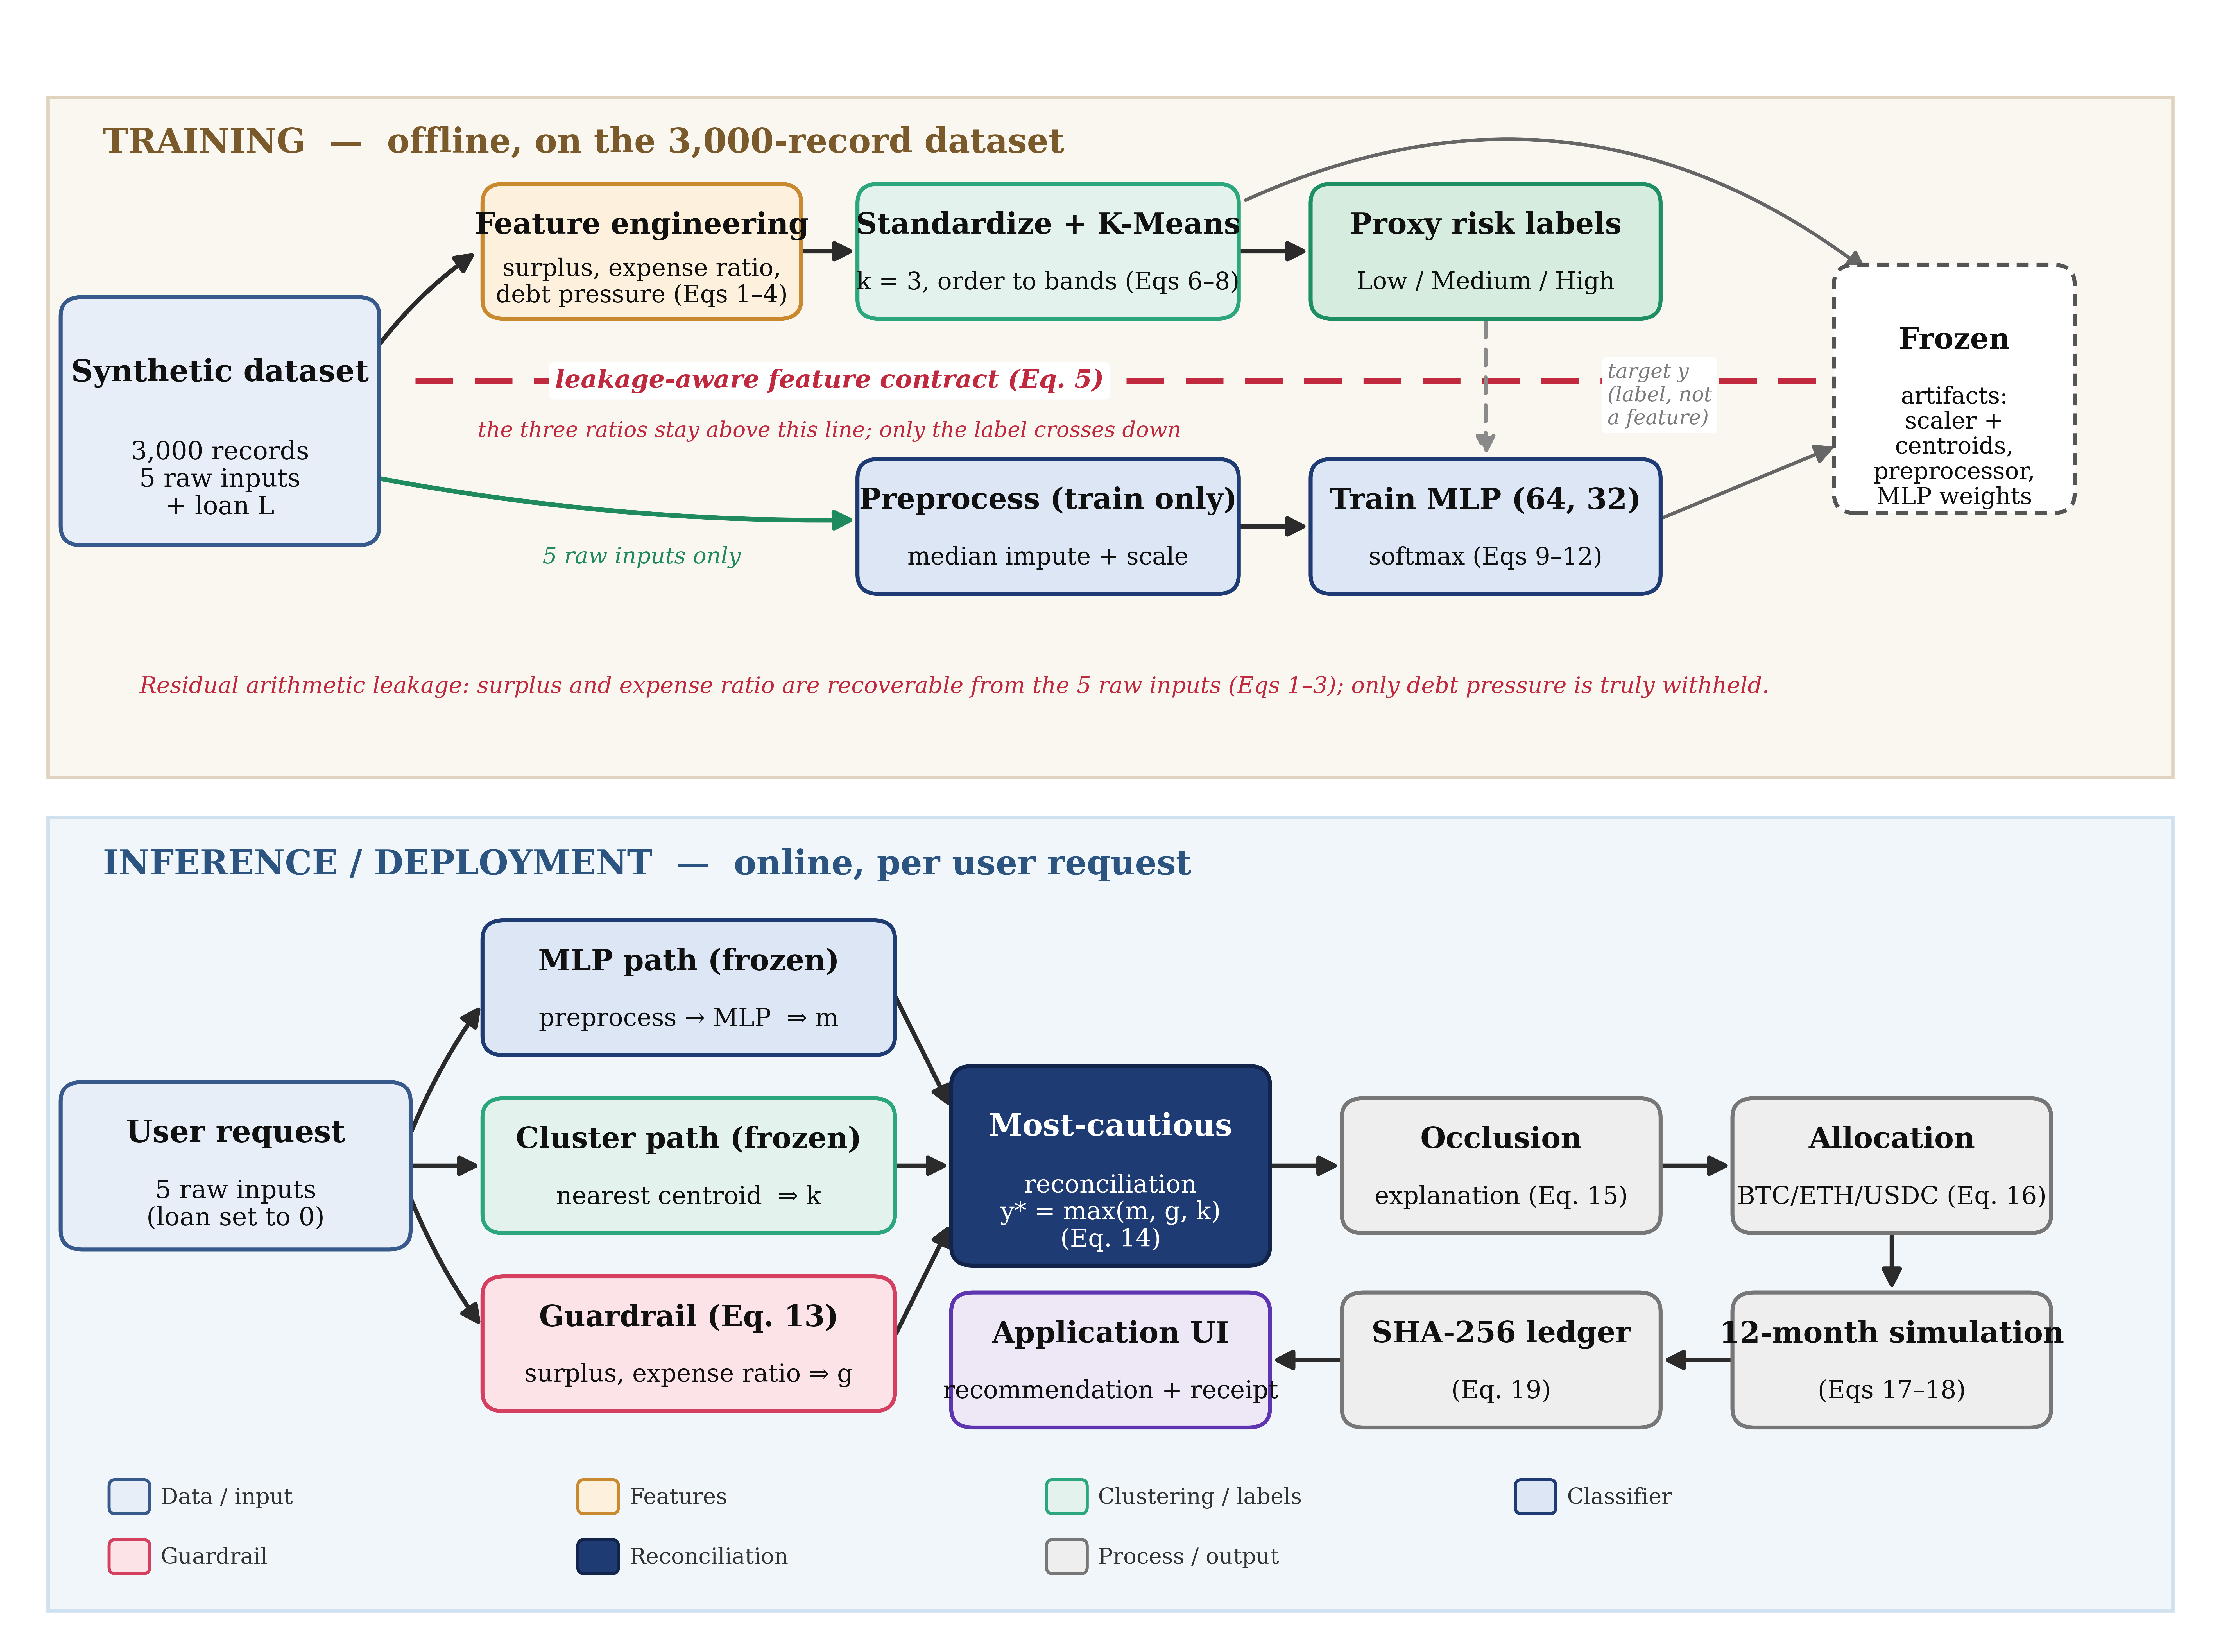
\includegraphics[width=\linewidth]{fig_architecture_v2.png}
\caption{End-to-end architecture, separated into the offline training pipeline (top)
and the online inference pipeline (bottom). During training the five raw inputs are
engineered into three ratios that are standardized and clustered ($k = 3$) to create
the proxy risk labels, whereas the classifier is trained on the five raw inputs only: a
leakage-aware feature contract (Eq.~\ref{eq:contract}) keeps the three ratios out of the
classifier feature matrix, and only the proxy label crosses that boundary, as the
supervised target. The fitted scaler, centroids, preprocessor, and network weights are
then frozen. At inference a user's inputs drive three parallel signals---the frozen MLP
($m$), the frozen cluster assignment ($k$), and the deterministic guardrail
($g$)---which are reconciled to the most cautious band $y^{*} = \max(m, g, k)$
(Eq.~\ref{eq:reconcile}), then explained by occlusion, mapped to a BTC/ETH/USDC
allocation, simulated over twelve months, and written to a hashed, verifiable ledger.}
\label{fig:arch}
\end{figure}

\subsection{Dataset and Provenance}\label{subsec:dataset}
The system is developed and evaluated on a synthetic personal-finance dataset of 3,000
records. The data are generated rather than collected, which permits controlled coverage
of financial scenarios but carries the external-validity caveat discussed in
Section~\ref{sec:discussion}. Two properties of the data are material to the evaluation
and are therefore stated plainly. First, although the file contains 3,000 rows, it holds
only 944 unique user identifiers, so roughly 95.8\% of rows are repeat observations of a
user already present elsewhere in the data; a naive row-level split therefore allows the
same individual to appear in both training and test partitions. Second, each record is
tagged with one of three macro scenarios---normal, inflation, or recession---which shapes
the distribution of incomes and expenses. Table~\ref{tab:dataset} summarizes the
composition and the train/test protocol.

\begin{table}[t]
\centering
\caption{Dataset composition and evaluation protocol}
\label{tab:dataset}
\begin{tabularx}{\linewidth}{@{}l L@{}}
\toprule
Property & Value \\
\midrule
Records / unique users & 3,000 / 944 ($\approx$95.8\% repeat rows) \\
Origin & Synthetic; 28 raw columns \\
Train / test split & 2,400 / 600 (80/20, seed 42) \\
Classifier inputs & 5 raw, user-facing fields \\
Cluster features & 3 engineered ratios \\
Proxy-label balance & Low 44.9\% $\cdot$ Medium 45.9\% $\cdot$ High 9.2\% \\
Scenario tag & normal / inflation / recession \\
Toolchain & scikit-learn 1.5.0, fixed seed \\
\bottomrule
\end{tabularx}
\end{table}

\begin{figure}[t]
\centering
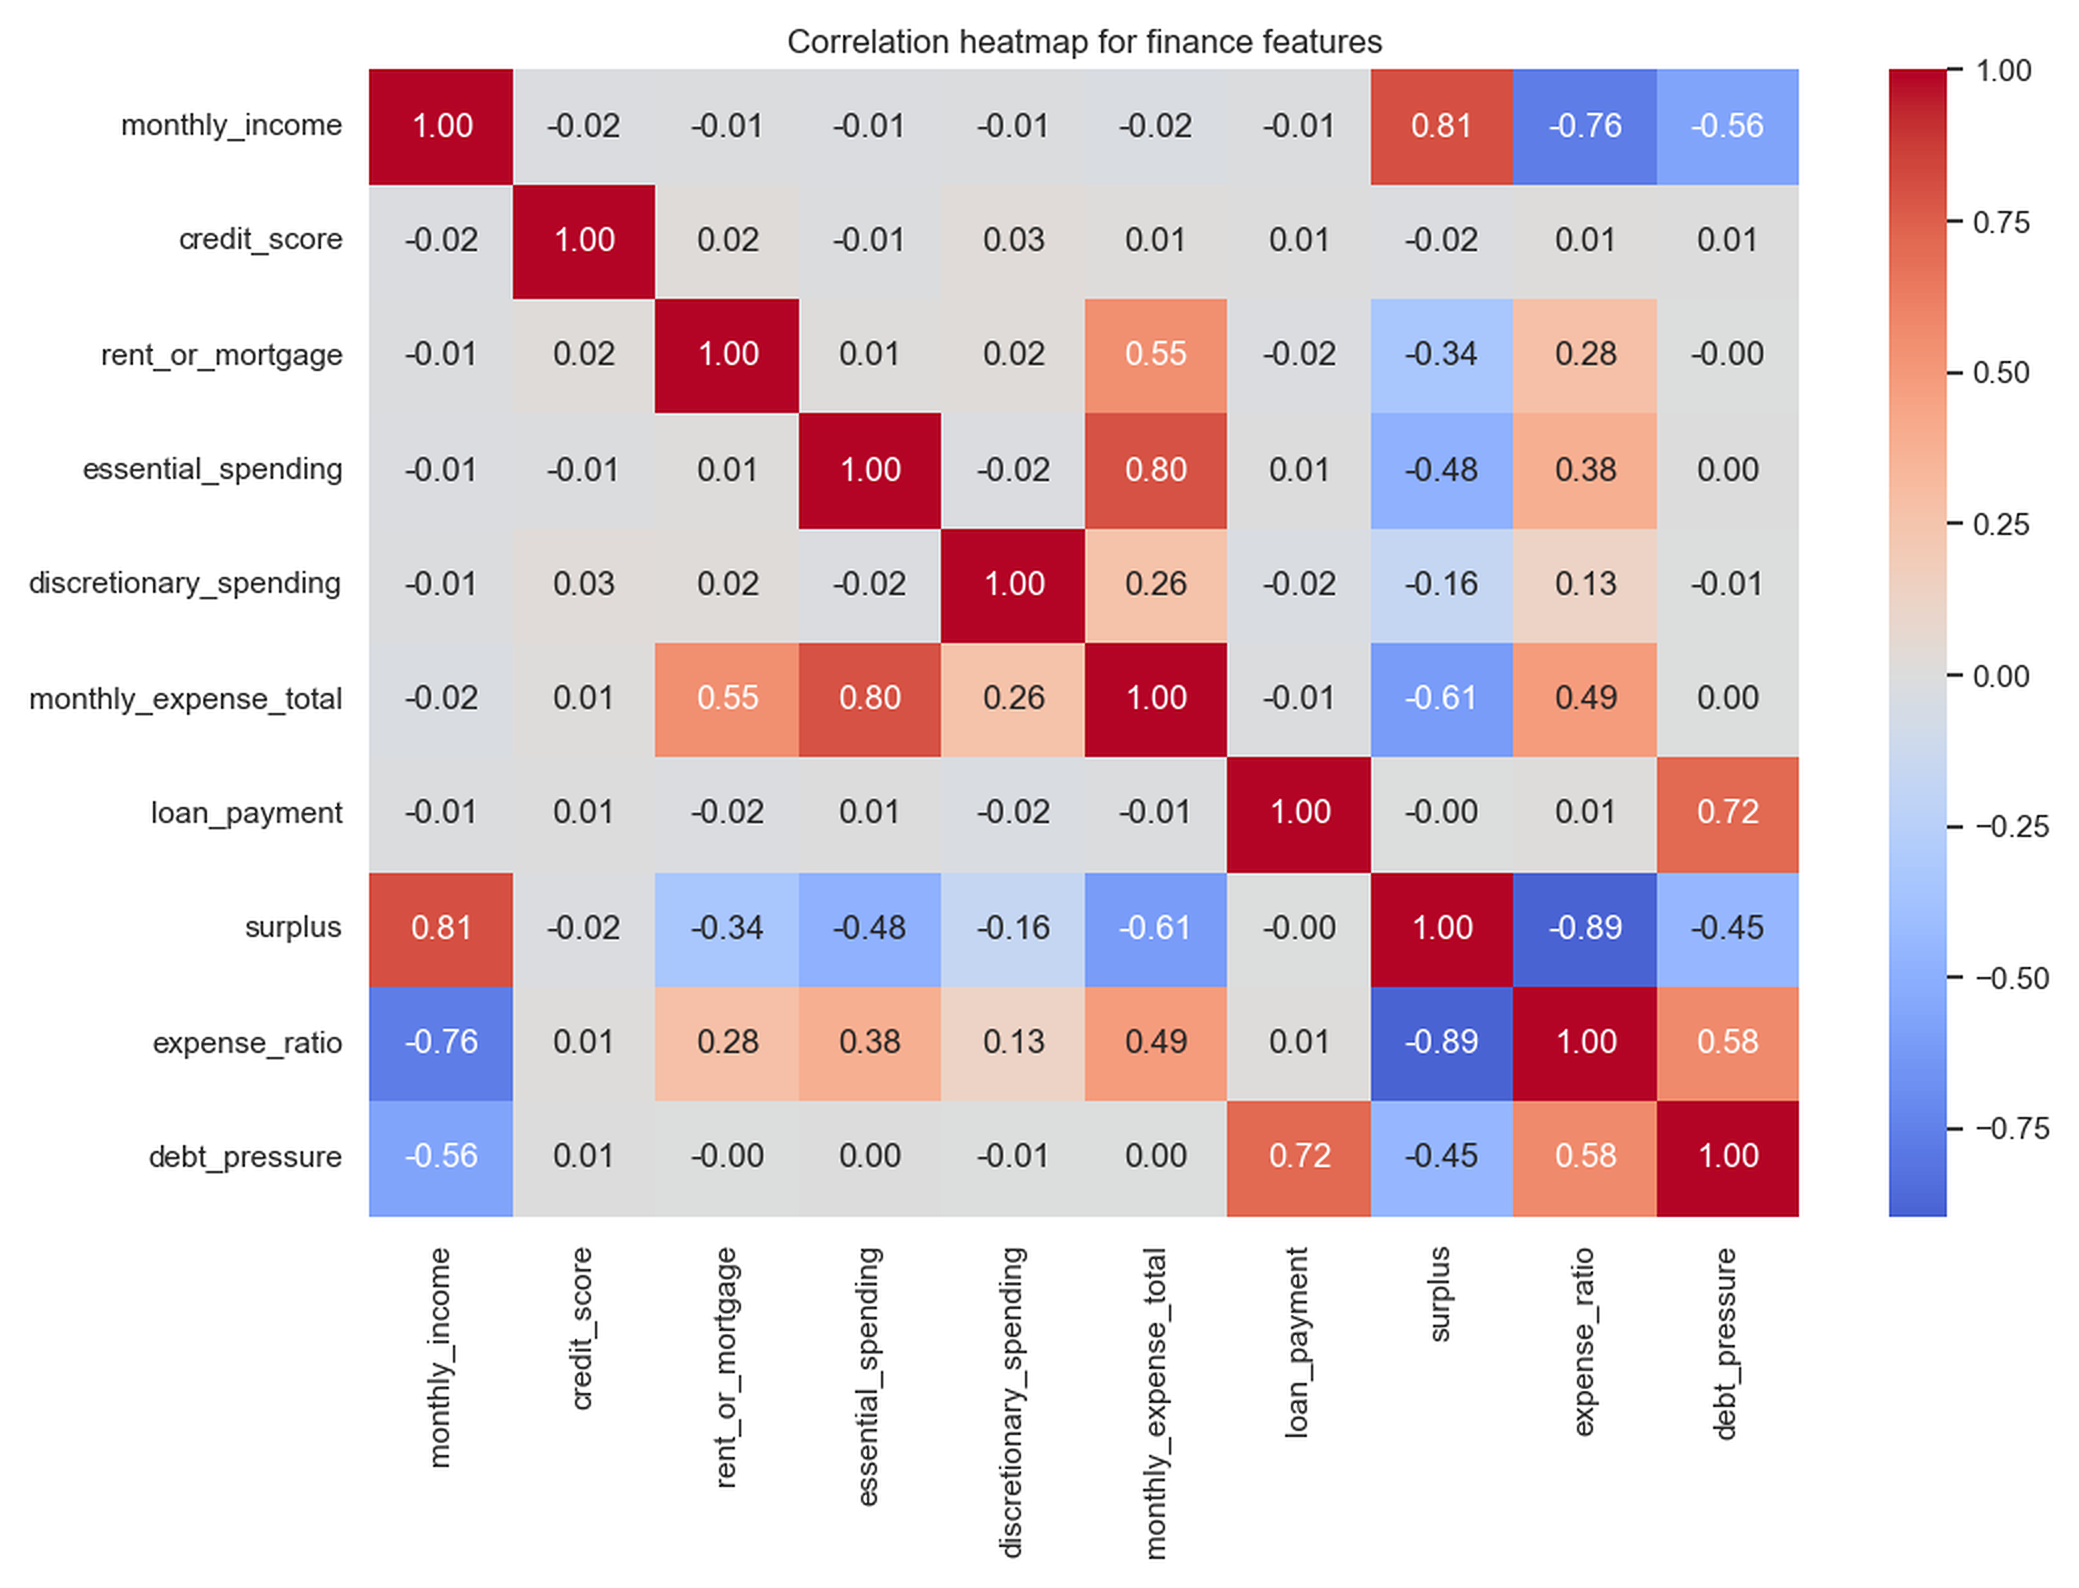
\includegraphics[width=0.55\linewidth]{fig_corr_heatmap.png}
\caption{Pearson correlation among the engineered financial quantities on the synthetic
data. Surplus and expense ratio are strongly anti-correlated ($-0.89$) and income and
surplus are strongly correlated (0.81), reflecting their shared algebraic origin.}
\label{fig:corr}
\end{figure}

\subsection{Feature Engineering}\label{subsec:feature-eng}
Each user supplies monthly income, a credit score, rent or mortgage, essential spending,
discretionary spending, and a loan payment. Total non-debt expenditure is the sum of the
three living-cost components, with the loan payment held out so that debt burden is not
double-counted:
\begin{equation}\label{eq:etotal}
E_{\text{total}} = R + S_{\text{ess}} + S_{\text{disc}}
\end{equation}
Monthly surplus is the income remaining after non-debt expenditure, and is the single
strongest indicator of financial headroom in the system:
\begin{equation}\label{eq:surplus}
\text{surplus} = I - E_{\text{total}}
\end{equation}
The expense ratio expresses non-debt cost as a percentage of income, so that a value at
or above 100\% signals that ordinary spending alone consumes the entire income:
\begin{equation}\label{eq:expratio}
\text{expense\_ratio} = (E_{\text{total}} / I) \times 100
\end{equation}
Debt pressure isolates the loan burden as a percentage of income:
\begin{equation}\label{eq:debt}
\text{debt\_pressure} = (L / I) \times 100
\end{equation}
In Equations~\eqref{eq:etotal}--\eqref{eq:debt}, $I$ is monthly income, $R$ rent or
mortgage, $S_{\text{ess}}$ and $S_{\text{disc}}$ essential and discretionary spending,
and $L$ the loan payment. When income is zero the two ratios are undefined, so the
implementation substitutes a fixed sentinel (999.0) that flags the record as an
extreme-risk outlier rather than dividing by zero. Table~\ref{tab:contract} lists every
variable together with the feature set it belongs to.

\subsection{The Leakage-Aware Feature Contract}\label{subsec:contract}
Because the three ratios are used to construct the labels, handing them to the classifier
would let it trivially recover its own target. The system therefore enforces a feature
contract that partitions the columns into a clustering set and a disjoint classifier set:
\begin{equation}\label{eq:contract}
F_{\text{clu}} \cap F_{\text{cls}} = \emptyset
\end{equation}
with $F_{\text{clu}}$ = \{surplus, expense\_ratio, debt\_pressure\} and $F_{\text{cls}}$
= \{monthly\_income, credit\_score, rent\_or\_mortgage, essential\_spending,
discretionary\_spending\}. A validation routine aborts training if any blocked column
reaches the classifier matrix. This column-level separation is real but incomplete, and
the system reports the gap rather than concealing it: because surplus and expense\_ratio
are algebraic functions of the classifier inputs
(Equations~\eqref{eq:etotal}--\eqref{eq:expratio}), two of the three clustering features
are exactly reconstructible from $F_{\text{cls}}$. Only debt\_pressure is truly withheld,
since it requires the loan payment, which is not a classifier input and is in fact set to
zero at inference. This residual arithmetic leakage is the principal reason a high
classification accuracy is attainable, and it is quantified in
Section~\ref{sec:discussion}.

\begin{table}[t]
\centering
\caption{Variables and the leakage-aware feature contract}
\label{tab:contract}
\begin{tabularx}{\linewidth}{@{}l L L >{\centering\arraybackslash}p{2.3cm}@{}}
\toprule
Symbol & Meaning & Feature set & Recoverable from $F_{\text{cls}}$ \\
\midrule
$I$ & Monthly income & Classifier & --- \\
credit & Credit score & Classifier & --- \\
$R$ & Rent / mortgage & Classifier & --- \\
$S_{\text{ess}}$ & Essential spending & Classifier & --- \\
$S_{\text{disc}}$ & Discretionary spending & Classifier & --- \\
$L$ & Loan payment & Input (zeroed at inference) & --- \\
surplus & $I - E_{\text{total}}$ & Cluster & Yes \\
expense\_ratio & $(E_{\text{total}} / I) \times 100$ & Cluster & Yes \\
debt\_pressure & $(L / I) \times 100$ & Cluster & No (needs $L$) \\
\bottomrule
\end{tabularx}
\end{table}

\subsection{Proxy Label Generation via Clustering}\label{subsec:clustering}
Because the data record no realized default or loss, risk labels are produced
unsupervised. The three ratios live on very different scales, so each is standardized to
zero mean and unit variance, with the statistics estimated on the training partition
only:
\begin{equation}\label{eq:standardize}
z_j = (x_j - \mu_j) / \sigma_j
\end{equation}
K-means then partitions the standardized vectors into $k$ clusters by minimizing the
within-cluster sum of squared Euclidean distances to the cluster centroids, assigning
each point to its nearest centroid:
\begin{equation}\label{eq:kmeans}
J = \sum_{i=1}^{k} \sum_{x \in C_i} \lVert x - \mu_i \rVert^2
\end{equation}
\begin{equation}\label{eq:assign}
c(x) = \arg\min_k \lVert x - \mu_k \rVert^2
\end{equation}
where $C_i$ is the set of points in cluster $i$, $\mu_i$ its centroid, and $J$ the
objective minimized. The cluster count is fixed at $k = 3$ to match the intended
Low/Medium/High banding. This is a documented trade-off rather than an assumption: a
two-cluster solution scores a higher silhouette (0.440), but two clusters cannot express
a three-band policy, so the three-cluster configuration (silhouette 0.370, adjusted Rand
index $0.868 \pm 0.064$ across resampling) is retained. Fitted clusters are ordered into
risk bands by profile---the highest-surplus cluster becomes Low risk and the
highest-expense-ratio cluster becomes High risk.

\subsection{Risk Classification}\label{subsec:classification}
A multilayer perceptron with two hidden layers of 64 and 32 units maps the classifier
feature vector to a risk band. Each hidden layer applies an affine transform and a
rectified-linear activation, and the output layer produces a distribution over the three
classes by softmax:
\begin{equation}\label{eq:h1}
h^{(1)} = \mathrm{ReLU}(W^{(1)}x + b^{(1)})
\end{equation}
\begin{equation}\label{eq:h2}
h^{(2)} = \mathrm{ReLU}(W^{(2)}h^{(1)} + b^{(2)})
\end{equation}
\begin{equation}\label{eq:softmax}
\hat{y}_c = \mathrm{softmax}(W^{(3)}h^{(2)} + b^{(3)})_c
\end{equation}
The network is trained by minimizing the multiclass cross-entropy between the predicted
distribution and the one-hot proxy label over the $N$ training examples:
\begin{equation}\label{eq:celoss}
L = -\frac{1}{N}\sum_{i=1}^{N}\sum_{c=1}^{3} y_{i,c}\log \hat{y}_{i,c}
\end{equation}
where $W^{(l)}$ and $b^{(l)}$ are the weights and biases of layer $l$, $\hat{y}_c$ the
predicted probability of class $c$, and $y_{i,c}$ the one-hot target. The configuration
of the clustering and classifier is given in Table~\ref{tab:config}.

\begin{table}[t]
\centering
\caption{Clustering and classifier configuration}
\label{tab:config}
\begin{tabularx}{\linewidth}{@{}l L@{}}
\toprule
Component & Setting \\
\midrule
Clustering & K-means, $k = 3$, n\_init = 50, seed 42 \\
Model search & K-means \& GMM ($k = 2$--$6$), DBSCAN---16 configs \\
Classifier & MLP, hidden (64, 32), ReLU, softmax(3) \\
Solver / regularization & Adam; L2, $\alpha = 0.001$ \\
Early stopping & val\_fraction 0.15, patience 20, max\_iter 1000 \\
Scaling & StandardScaler fitted on train only \\
\bottomrule
\end{tabularx}
\end{table}

\subsection{Rule-Based Safety Guardrail}\label{subsec:guardrail}
A statistical prediction alone is not a safe basis for advice, so the classifier output
passes through a deterministic guardrail that encodes conservative cash-flow rules and
can only ever raise concern:
\begin{equation}\label{eq:guardrail}
g = \begin{cases}
2 & \text{if } (\text{surplus} < 0 \ \lor\ \text{expense\_ratio} \geq 90),\\
1 & \text{if } \text{expense\_ratio} \geq 60,\\
0 & \text{otherwise.}
\end{cases}
\end{equation}
where 0, 1, and 2 denote Low, Medium, and High risk. A user whose spending exceeds
income, or whose expense ratio reaches 90\%, is treated as High risk irrespective of the
model. The deployed guardrail routine additionally escalates on debt pressure---to High
when debt\_pressure $\geq$ 35\% and to Medium when debt\_pressure $\geq$ 20\%---but on
this dataset those branches are almost entirely subsumed by the cash-flow conditions:
including them leaves the guardrail-only High share unchanged at 60.6\% and shifts the
Low/Medium split by under 0.2 percentage points, so \eqref{eq:guardrail} states the
cash-flow conditions that drive the analysis in Section~\ref{subsec:guardrail-dom}. A
separate recommender module applies a different medium-risk threshold (75 rather than
60); this inconsistency is disclosed as a limitation in Section~\ref{sec:discussion}.

\subsection{Most-Cautious Reconciliation}\label{subsec:reconciliation}
The final band reconciles the model prediction $m$, the guardrail $g$, and the cluster
assignment $k$ by taking the most cautious of the three under the order Low $<$ Medium
$<$ High:
\begin{equation}\label{eq:reconcile}
y^{*} = \max(m, g, k)
\end{equation}
This guarantees that the assessed risk is never lower than any individual signal implies,
so neither a classifier error nor an optimistic cluster can yield an unsafely low
recommendation. Section~\ref{sec:results} quantifies how often each signal is decisive;
the guardrail is the binding signal for most users.

\subsection{Model-Adaptive Explanation}\label{subsec:explanation}
To explain a decision, the system measures how sensitive the predicted probability is to
each input. For the deployed MLP, which exposes no linear coefficients, the influence of
feature $j$ is estimated by occlusion: the feature is replaced by its mean and the
resulting drop in the predicted probability of the assigned class $\hat{c}$ is recorded:
\begin{equation}\label{eq:occlusion}
\Delta_j = \hat{y}_{\hat{c}}(x) - \hat{y}_{\hat{c}}(x_{-j})
\end{equation}
A large influence means the feature strongly supported the prediction. The strategy is
model-adaptive---a linear model would instead report signed coefficients and a tree
ensemble impurity importances---but for the deployed network the mean-imputation
occlusion branch is the one actually exercised. This is an occlusion-based sensitivity
method; it is neither SHAP nor a partial-derivative sensitivity method, and is not
described as such.

\subsection{Risk-Aligned Allocation}\label{subsec:allocation}
The reconciled band maps deterministically to a fixed Bitcoin/Ethereum/USDC allocation
that scales crypto exposure down and stablecoin weighting up as risk rises:
\begin{equation}\label{eq:alloc}
w(\text{Low}) = (35, 35, 30);\quad w(\text{Med}) = (20, 20, 60);\quad w(\text{High}) =
(0, 0, 100)
\end{equation}
with weights in percent summing to 100. A High-risk user is placed entirely in the USDC
stablecoin, a choice motivated by the DeFi-instability literature reviewed in
Section~\ref{sec:related}.

\subsection{Deterministic Twelve-Month Simulation}\label{subsec:simulation}
The allocation is evaluated by compounding an initial capital over twelve months using a
fixed monthly return series for each asset. The portfolio value evolves as
\begin{equation}\label{eq:portfolio}
V_t = V_{t-1}\cdot\left(1 + \sum_a w_a\, r_{a,t}\right)
\end{equation}
and the return over the horizon is the total growth relative to the initial capital:
\begin{equation}\label{eq:roi}
\mathrm{ROI} = (V_{12} - V_0)/V_0
\end{equation}
where $V_t$ is the value at month $t$ ($V_0$ the initial capital), $w_a$ the weight of
asset $a$, and $r_{a,t}$ its fixed monthly return. Because the returns are hardcoded
constants rather than sampled or historical series, this is a deterministic scenario
projection, not a market backtest. The originally reported ROI figures were affected by
an off-by-one normalization (dividing by the first simulated month rather than the
initial capital); Section~\ref{sec:results} reports the corrected values.

\subsection{Tamper-Evident Audit Logging}\label{subsec:audit-log}
Every recommendation is recorded in a tamper-evident ledger. The payload is serialized
into a canonical form with sorted keys and hashed with SHA-256:
\begin{equation}\label{eq:hash}
H = \text{SHA-256}(\,\text{serialize}(\text{payload}, \text{sorted})\,)
\end{equation}
The digest is stored with a unique transaction identifier; integrity verification
re-serializes and re-hashes the stored payload and compares it against $H$, so any
alteration is detectable. The ledger labels entries as a simulated testnet and runs in
memory---it is not deployed to a live blockchain, a limitation revisited in
Section~\ref{sec:discussion}.

% =====================  SECTION IV  =====================
\section{Experimental Setup and Results}\label{sec:results}

This section reports what the system was measured to do. To keep the evidential status of
each figure explicit, results are labeled as one of four kinds: an experimental result
(measured on held-out data), a system output (a value the pipeline emits by
construction), a simulation result (an outcome of the deterministic projection), or a
theoretical property (a guarantee that follows from the design). Every quantitative claim
is drawn from the verified metric artifacts.

\subsection{Experimental Setup}\label{subsec:setup}
All models were trained with scikit-learn 1.5.0 under a fixed random seed for
reproducibility, using the configuration in Table~\ref{tab:config}. Headline metrics are
computed on a stratified 20\% holdout of 600 records; stability is estimated with
stratified five-fold cross-validation in which the clustering is refitted inside each
fold so that no proxy-label information crosses the split. Uncertainty on the headline
metrics is quantified by a bootstrap 95\% confidence interval. The proxy-label
distribution is imbalanced---Low 44.9\%, Medium 45.9\%, High 9.2\%---which is the
backdrop against which the minority High-risk results should be read.

\subsection{Clustering Quality}\label{subsec:clustering-quality}
\textbf{\textit{Experimental result.}} The chosen three-cluster solution attains a
silhouette coefficient of 0.370, a Calinski--Harabasz index of 2158.37, and a
Davies--Bouldin index of 0.925 on the standardized ratios, with assignments stable under
resampling at an adjusted Rand index of $0.868 \pm 0.064$. The three clusters map onto
financially distinct, monotonically ordered groups, which supports their use as risk
proxies: as Table~\ref{tab:cluster} shows, mean surplus falls and mean expense ratio
rises steadily from the Low to the High band. Fig.~\ref{fig:cluster} shows the separation
in principal-component space and in surplus--expense-ratio space with the guardrail
thresholds overlaid.

\begin{table}[t]
\centering
\caption{Mean financial profile of each risk cluster (system output)}
\label{tab:cluster}
\begin{tabularx}{\linewidth}{@{}l C C C@{}}
\toprule
Risk band & Mean surplus & Mean expense ratio & Mean debt pressure \\
\midrule
Low & $+1171.67$ & 76.04\% & 10.43\% \\
Medium & $-583.14$ & 117.76\% & 14.30\% \\
High & $-1994.60$ & 195.80\% & 27.54\% \\
\bottomrule
\end{tabularx}
\par\vspace{3pt}
{\footnotesize\itshape\raggedright The debt-pressure column is informative for profiling
but is set to zero on the guardrail path at inference; the clusters themselves are formed
on all three ratios.\par}
\end{table}

\begin{figure}[t]
\centering
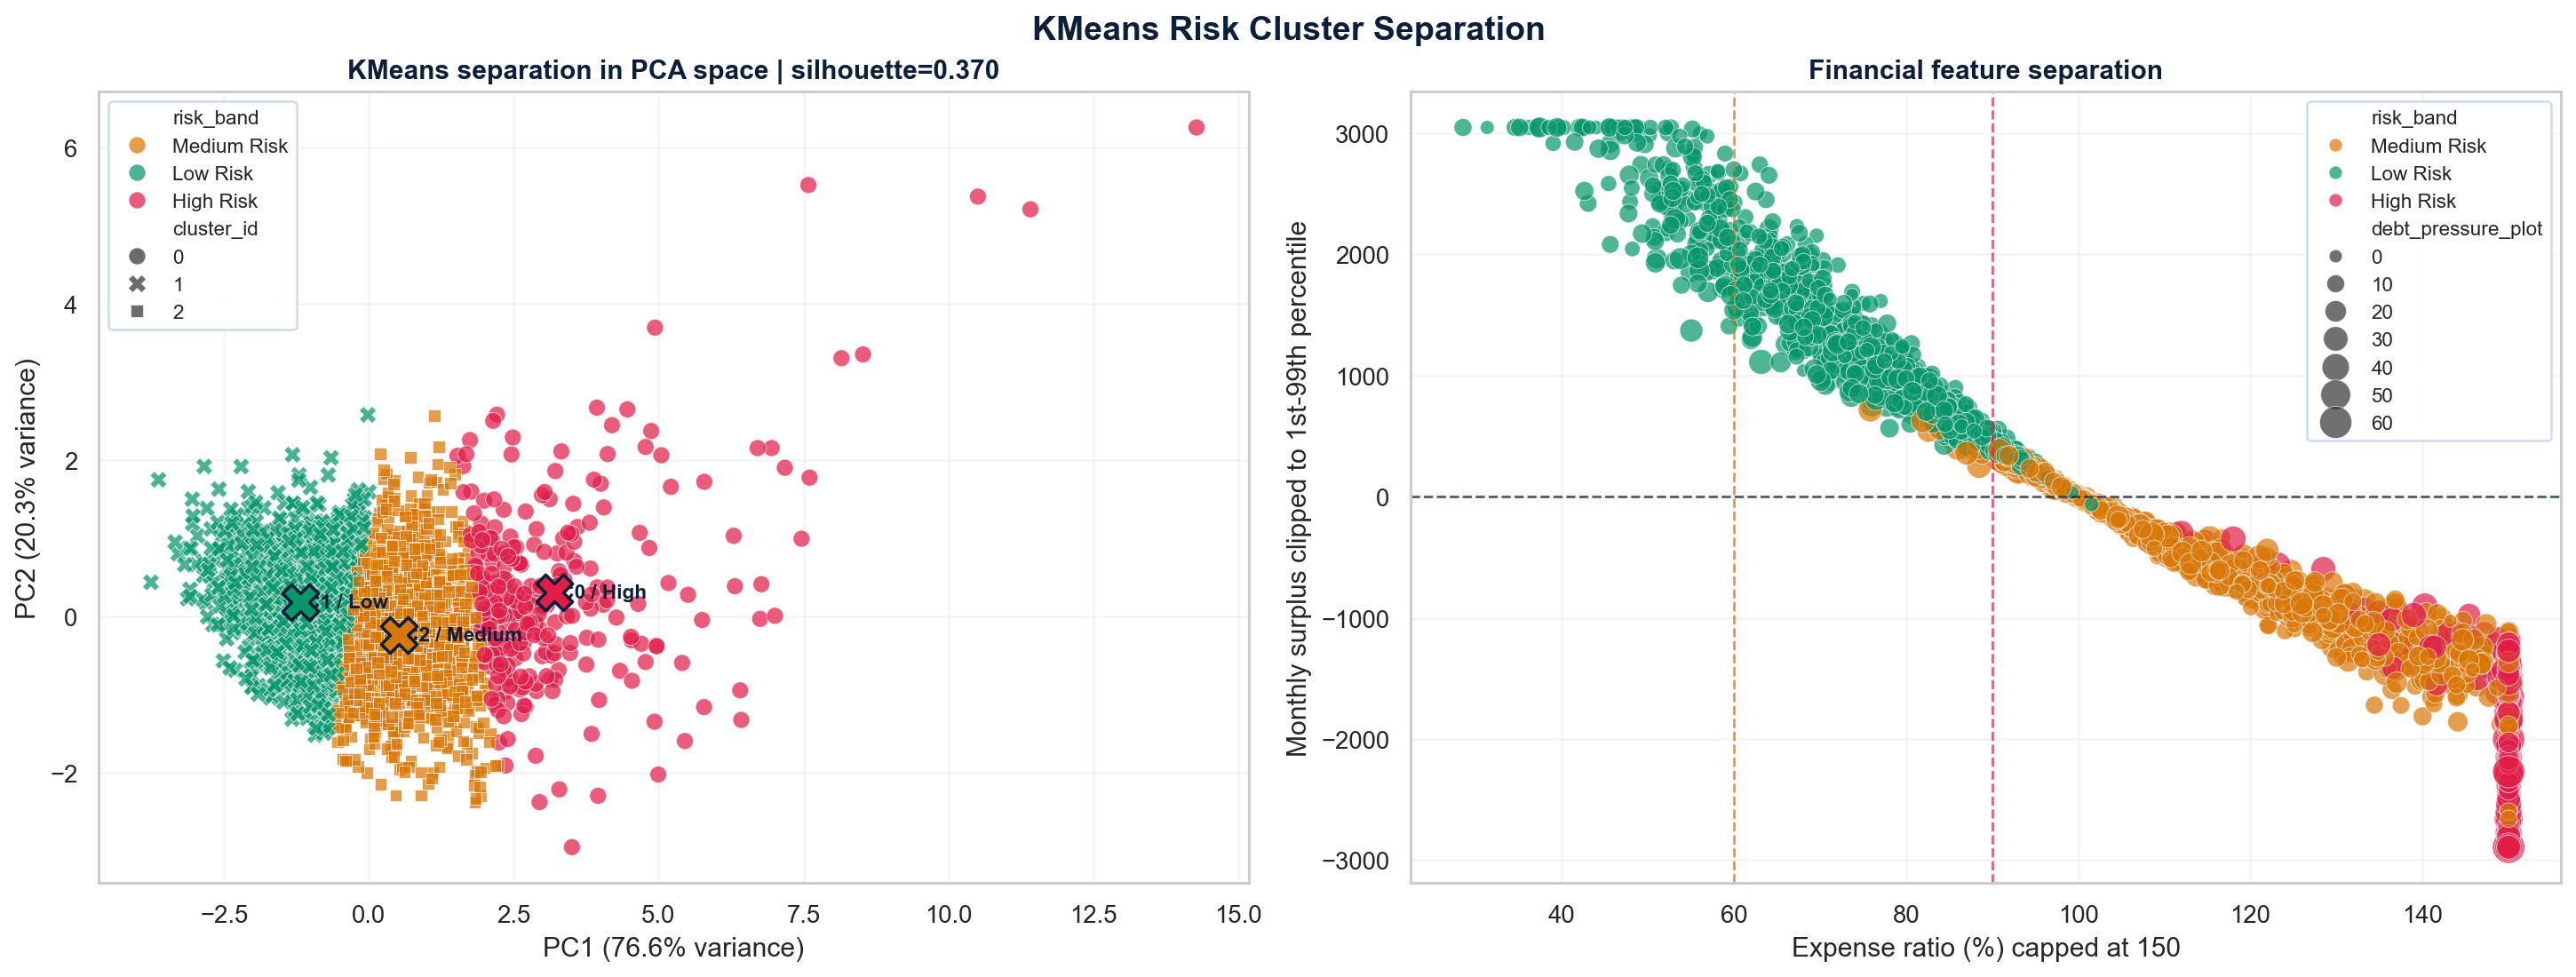
\includegraphics[width=\linewidth]{fig_cluster_sep.png}
\caption{K-means separation of the three risk segments (silhouette 0.370). Left: the
first two principal components. Right: the same users in surplus--expense-ratio space with
guardrail thresholds overlaid.}
\label{fig:cluster}
\end{figure}

\subsection{Classification Performance}\label{subsec:classification-perf}
\textbf{\textit{Experimental result.}} On the 600-record holdout the MLP attains 91.0\%
accuracy and a 0.881 macro-F1, with a macro one-vs-rest ROC-AUC of 0.986 and a macro
PR-AUC of 0.951. Five-fold cross-validation gives 91.2\% $\pm$ 0.9\% accuracy and
$0.867 \pm 0.018$ macro-F1, so the holdout figure is representative rather than a
favorable split, and a bootstrap 95\% confidence interval places holdout accuracy in
[0.888, 0.933] and macro-F1 in [0.847, 0.912]. Performance is uneven across bands
(Table~\ref{tab:perclass}): the model is strong on the well-represented Low and Medium
bands but markedly weaker on the minority High band, whose F1 of 0.791 reflects its small
support (62 cases) and its overlap with the Medium band.

\begin{table}[t]
\centering
\caption{Per-class classifier performance of the deployed MLP on the holdout
(experimental result)}
\label{tab:perclass}
\begin{tabularx}{\linewidth}{@{}l C C C C@{}}
\toprule
Risk band & Precision & Recall & F1 score & Support \\
\midrule
Low & 0.922 & 0.971 & 0.946 & 242 \\
Medium & 0.935 & 0.878 & 0.906 & 296 \\
High & 0.761 & 0.823 & 0.791 & 62 \\
\midrule
Macro average & 0.873 & 0.891 & 0.881 & 600 \\
Weighted average & 0.912 & 0.910 & 0.910 & 600 \\
\bottomrule
\end{tabularx}
\par\vspace{3pt}
{\footnotesize\itshape\raggedright Precision, recall, and F1 are computed directly from
the MLP confusion matrix in Fig.~\ref{fig:cm}(a); the macro average is unweighted across
classes and the weighted average is weighted by support. Weighted recall equals overall
accuracy (0.910) by construction.\par}
\end{table}

Fig.~\ref{fig:cm} shows the confusion matrix of every evaluated model on the identical
600-case holdout, which exposes the error structure that the aggregate scores hide. Three
properties hold across all four models. First, errors are overwhelmingly single-band
confusions between adjacent classes. Second---and this matters for a conservative
advisory system---not one model ever confuses Low risk with High risk in either
direction: both off-diagonal corners are exactly zero for the MLP, logistic regression,
random forest, and decision tree alike, so on the classifier path the system never
commits the catastrophic inversion of calling a high-risk user low-risk or vice versa.
Third, the residual errors concentrate in the Medium band and at the Medium--High
boundary, which is precisely where the deterministic guardrail is positioned to intervene.

The minority High band is where the models differ most, and the comparison does not favor
the MLP. Reading recall along the High row of Fig.~\ref{fig:cm}, logistic regression
recovers 61 of 62 true High-risk users (recall 0.984), against 51 of 62 for both the MLP
and the random forest (0.823) and 54 of 62 for the decision tree (0.871). Logistic
regression attains this by escalating more readily---it also relabels 36 Medium users as
High---so its High-band precision falls to 0.629 against the MLP's 0.761, the familiar
precision--recall trade-off on a small class. For a safety-first system that would rather
over- than under-state risk, the higher High-risk sensitivity of logistic regression is
arguably the more desirable operating point, which further weakens any case for preferring
the neural model on the minority class. The per-class ROC and precision--recall curves for
the MLP in Fig.~\ref{fig:rocpr} corroborate the aggregate picture: near-perfect
separability on the well-supported Low band and a visibly lower precision--recall area on
the 62-case High band.

\begin{figure}[t]
\centering
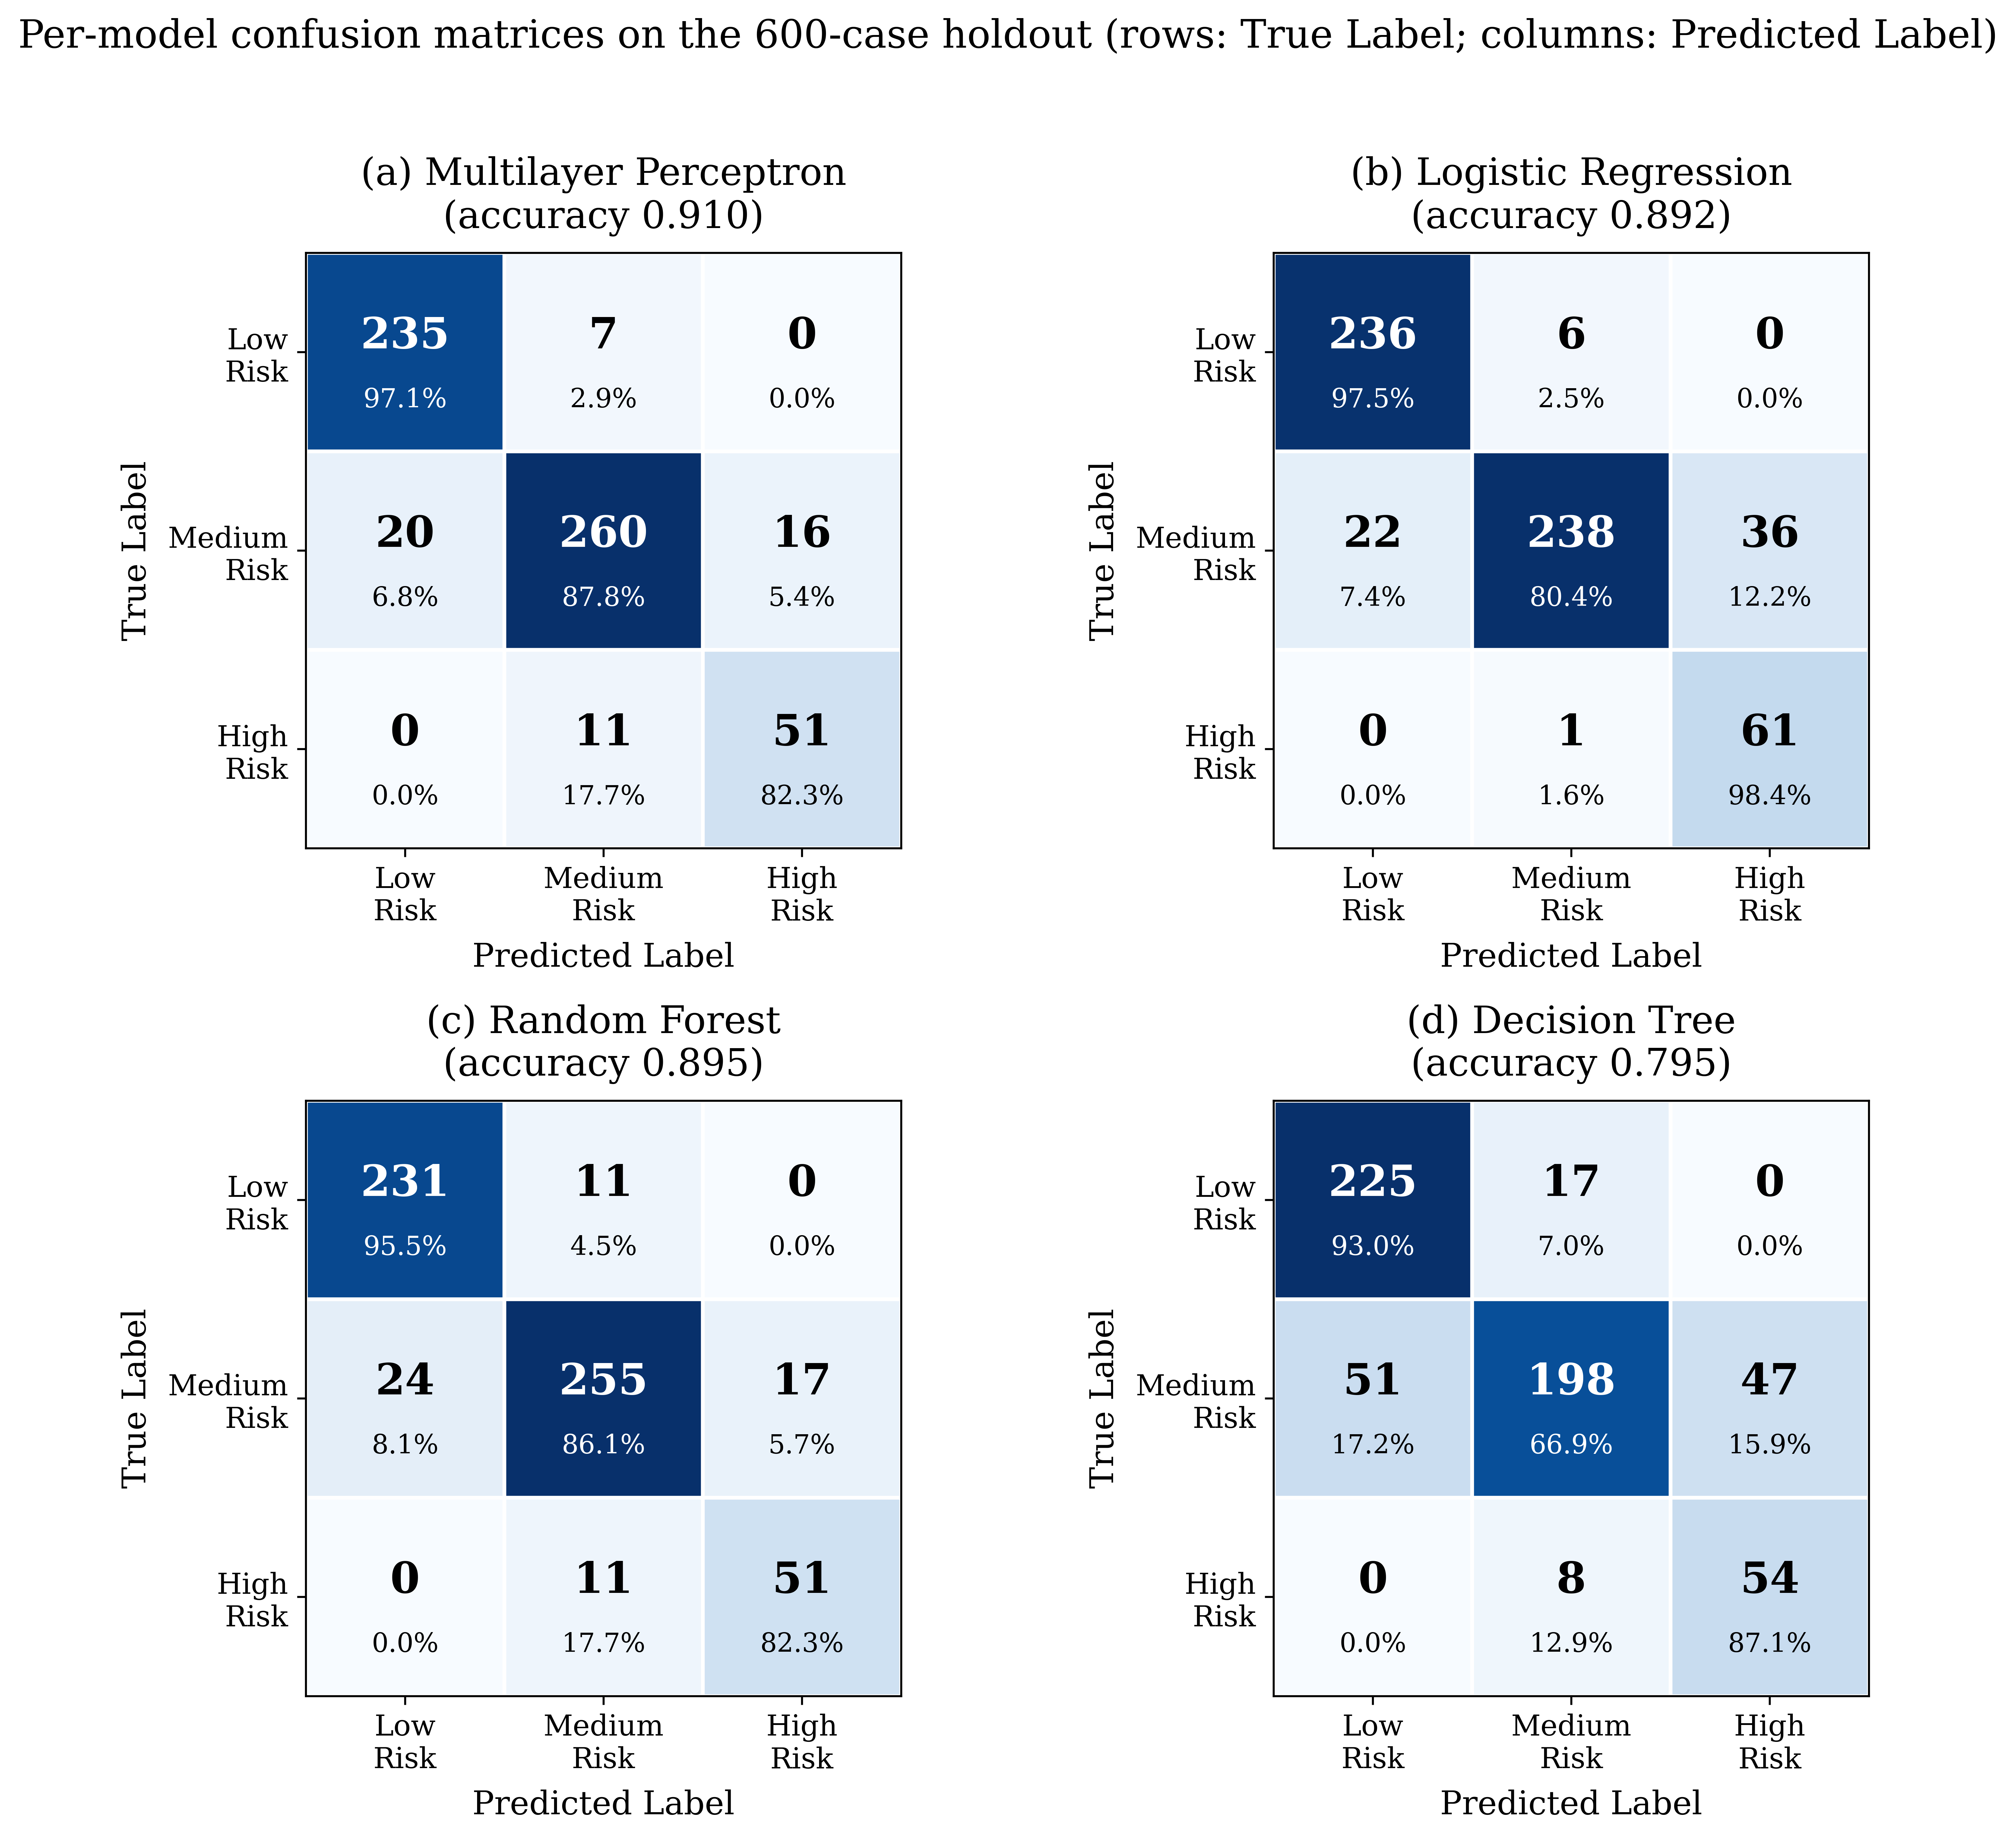
\includegraphics[width=\linewidth]{fig_confusion_all.png}
\caption{Confusion matrices of all four evaluated classifiers on the identical 600-case
holdout (rows: true label; columns: predicted label; each cell shows the count and the
row percentage). Errors are confined to adjacent bands and no model produces any
Low$\leftrightarrow$High confusion. All four panels are computed from the same held-out
predictions and ground-truth proxy labels used for
Tables~\ref{tab:perclass}--\ref{tab:stats}, and reproduce the accuracy and macro-F1 of
Table~\ref{tab:modelcompare} exactly.}
\label{fig:cm}
\end{figure}

\begin{figure}[t]
\centering
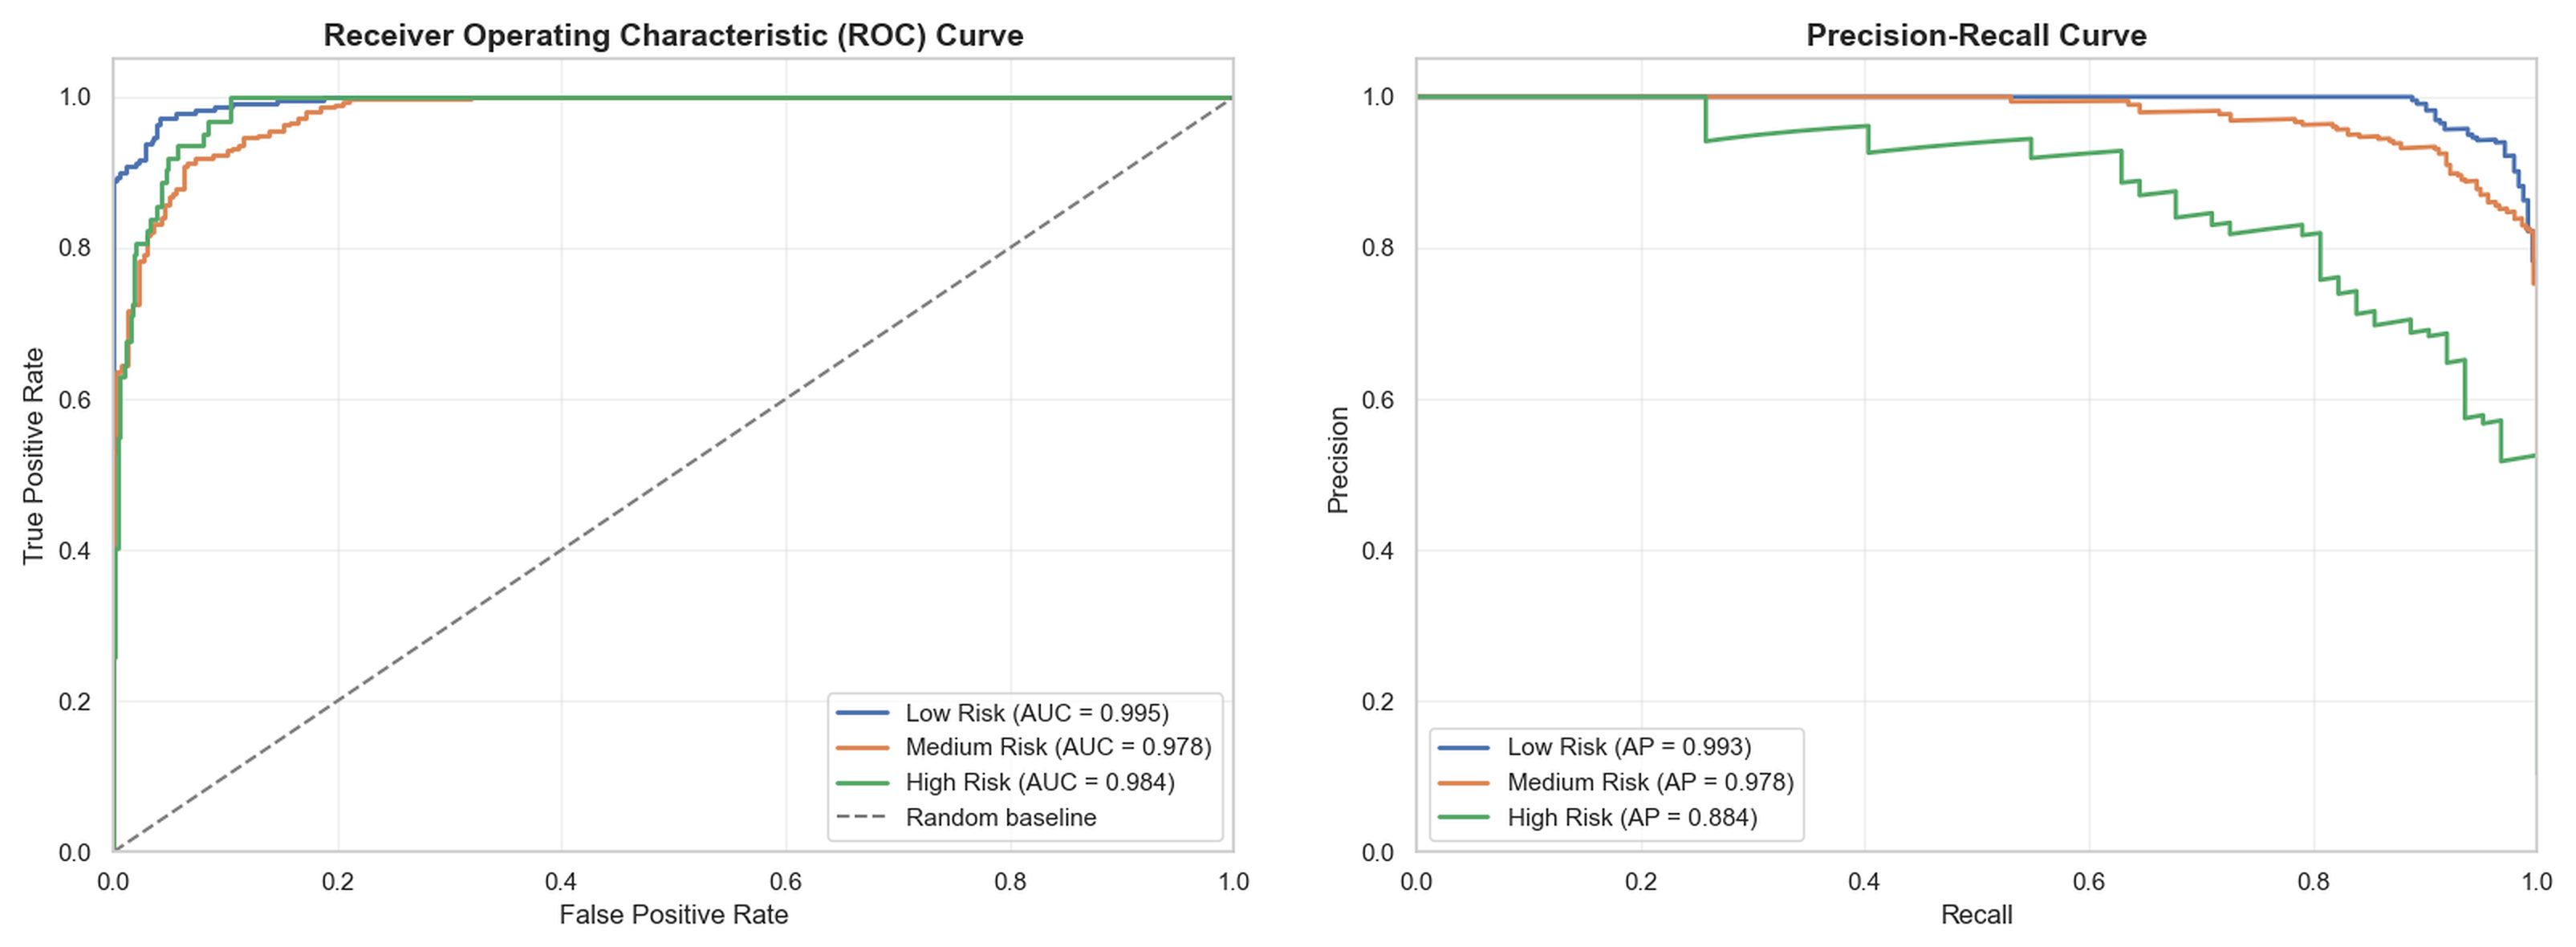
\includegraphics[width=\linewidth]{fig_roc_pr.png}
\caption{Per-class one-vs-rest ROC curves (left) and precision--recall curves (right) for
the MLP. The High-risk band shows the lowest average precision.}
\label{fig:rocpr}
\end{figure}

\subsection{Comparative Analysis}\label{subsec:comparative-analysis}
\textbf{\textit{Experimental result.}} The MLP was compared against logistic regression, a
decision tree, and a random forest under the same protocol
(Table~\ref{tab:modelcompare}, Fig.~\ref{fig:modelcompare}). The MLP leads on accuracy and
macro-F1, but the margin over the two strongest baselines is slight, and logistic
regression in fact marginally exceeds the MLP on both macro ROC-AUC (0.9861 vs.\ 0.9859)
and macro PR-AUC (0.9520 vs.\ 0.9514)---an inversion to which an accuracy/F1 selection
rule is blind. Only the decision tree is clearly behind.

\begin{table}[t]
\centering
\caption{Model comparison on the holdout set (experimental result)}
\label{tab:modelcompare}
\begin{tabularx}{\linewidth}{@{}l C C C C@{}}
\toprule
Model & Accuracy & Macro-F1 & ROC-AUC & PR-AUC \\
\midrule
MLP (deployed) & 0.910 & 0.881 & 0.9859 & 0.9514 \\
Logistic regression & 0.892 & 0.864 & 0.9861 & 0.9520 \\
Random forest & 0.895 & 0.868 & 0.9764 & 0.9233 \\
Decision tree & 0.795 & 0.765 & 0.9276 & 0.8359 \\
\bottomrule
\end{tabularx}
\end{table}

\begin{figure}[t]
\centering
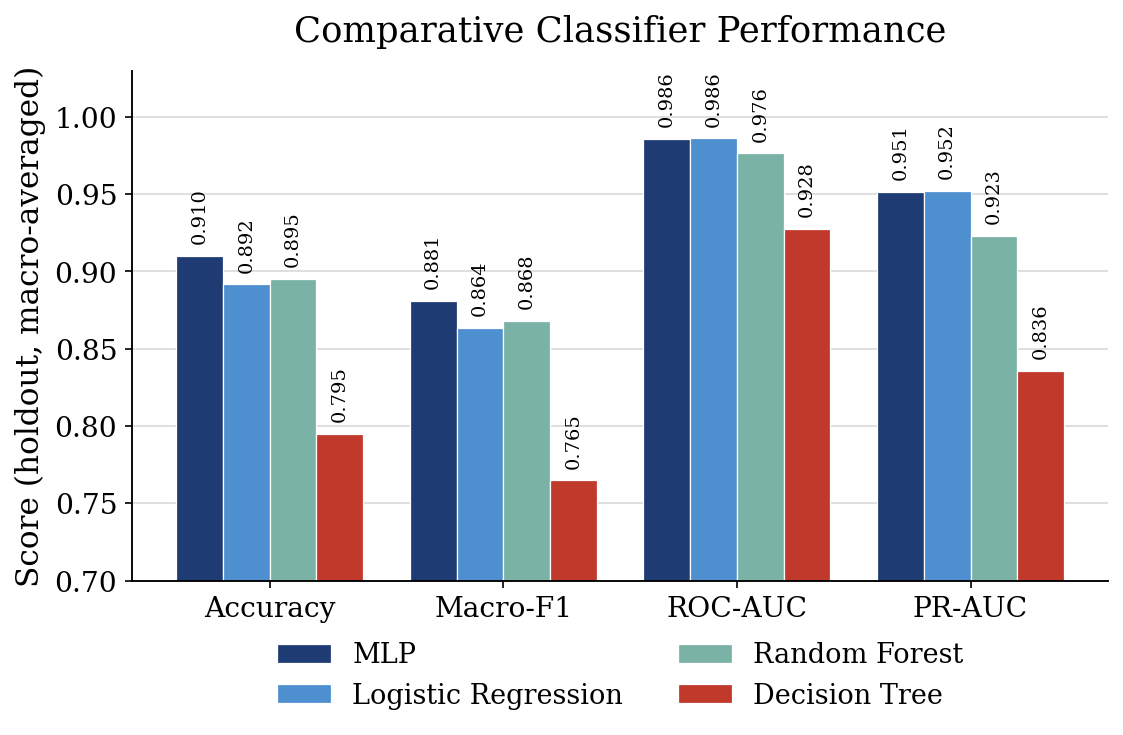
\includegraphics[width=0.72\linewidth]{fig_model_compare_v2.png}
\caption{Accuracy, macro-F1, ROC-AUC, and PR-AUC for the four classifiers. The MLP and
logistic regression are statistically indistinguishable on this dataset (see
Table~\ref{tab:stats}).}
\label{fig:modelcompare}
\end{figure}

\subsection{Statistical Validation}\label{subsec:statistical}
\textbf{\textit{Experimental result.}} Because every classifier was evaluated on the same
600-case holdout with an identical class ordering, model differences can be tested on
paired predictions. For each pairwise comparison the null hypothesis is that the two
models have equal population error rates---equivalently, that their discordant predictions
are symmetric---against the two-sided alternative of unequal error rates, at a significance
level of $\alpha = 0.05$. McNemar's test is the appropriate paired test for this design;
it is computed with a continuity correction, and for the small discordant counts here an
exact binomial test yields the same decisions. Table~\ref{tab:stats} reports each
comparison against the deployed MLP.

The MLP is not statistically distinguishable from logistic regression ($\chi^2 = 2.70$ on
24/13 discordant pairs, $p = 0.100$) or from the random forest ($\chi^2 = 1.83$ on 22/13
pairs, $p = 0.176$) at $\alpha = 0.05$; only the decision tree is beaten significantly
($\chi^2 = 48.67$ on 82/13 pairs, $p < 0.001$). The discordant-pair odds ratios---a
McNemar effect-size measure---are correspondingly modest for the two close baselines (1.85
and 1.69) and large only for the decision tree (6.31). Because three comparisons are made
against the same MLP, a Holm--Bonferroni correction is applied across them; it leaves
every decision unchanged, since the decision-tree result stays below its adjusted
threshold while the logistic-regression and random-forest results stay above theirs.

These tests are read alongside the interval estimates. The headline metrics carry a
bootstrap 95\% confidence interval computed over 300 resamples of the holdout: holdout
accuracy has a point estimate of 0.910 with a 95\% interval of [0.888, 0.933], and
macro-F1 a point estimate of 0.881 with a 95\% interval of [0.847, 0.912]. Five-fold
stratified cross-validation is consistent with these figures (accuracy
$0.912 \pm 0.009$, macro-F1 $0.867 \pm 0.018$). The overlapping intervals and the
non-significant tests together mean the evidence does not support a claim that a neural
model is necessary for this task; the MLP is retained for its probability outputs, which
the occlusion explainer consumes, and the non-significant comparisons are reported as an
absence of demonstrated superiority rather than as proof of equivalence.

\begin{table}[t]
\centering
\caption{Statistical validation of pairwise model differences (experimental result)}
\label{tab:stats}
\footnotesize
\setlength{\tabcolsep}{3pt}
\begin{tabularx}{\linewidth}{@{}L c c c c c L@{}}
\toprule
Comparison & Test & $\chi^2$ (b/c) & $p$-value & $\alpha$ & Significant? & Interpretation \\
\midrule
MLP vs.\ logistic regression & McNemar & 2.70 (24/13) & 0.100 & 0.05 & No & No demonstrated difference \\
MLP vs.\ random forest & McNemar & 1.83 (22/13) & 0.176 & 0.05 & No & No demonstrated difference \\
MLP vs.\ decision tree & McNemar & 48.67 (82/13) & $<$ 0.001 & 0.05 & Yes & MLP significantly better \\
\bottomrule
\end{tabularx}
\par\vspace{3pt}
{\footnotesize\itshape\raggedright $\chi^2$ is McNemar's statistic with continuity
correction and (b/c) are the discordant-pair counts---cases the MLP classifies correctly
and the comparator does not (b), versus the reverse (c). All $p$-values are two-sided; the
`Significant?' decision reflects the Holm--Bonferroni-adjusted threshold, which coincides
with the uncorrected decision here.\par}
\end{table}

\subsection{Guardrail Dominance and Reconciliation}\label{subsec:guardrail-dom}
\textbf{\textit{System output.}} Applied across the dataset, the guardrail alone assigns
5.87\% of users to Low, 33.53\% to Medium, and 60.60\% to High risk. The guardrail signal
is greater than or equal to the cluster signal for 100\% of users and strictly greater for
84.13\%, so the guardrail---not the classifier---is the binding signal in the
reconciliation for most users. Read the other way (Fig.~\ref{fig:guardrail}), when the
model predicts Low its prediction never changes the final band (0.00\% of cases), when it
predicts Medium the final band changes for 5.87\% of cases, and when it predicts High it
changes for 39.40\%. Substituting a constant Low-risk predictor would alter 0.00\% of
final decisions.

This is the single most consequential finding, and it qualifies a naive reading of the
91\% accuracy. Because the conservative guardrail escalates so many users to High risk on
cash-flow grounds alone, the learned classifier determines the end recommendation for only
a minority of users. The accuracy is a genuine property of the classifier, but it is not a
measure of the system's end-to-end decision quality, which is dominated by the
deterministic layer.

\begin{figure}[t]
\centering
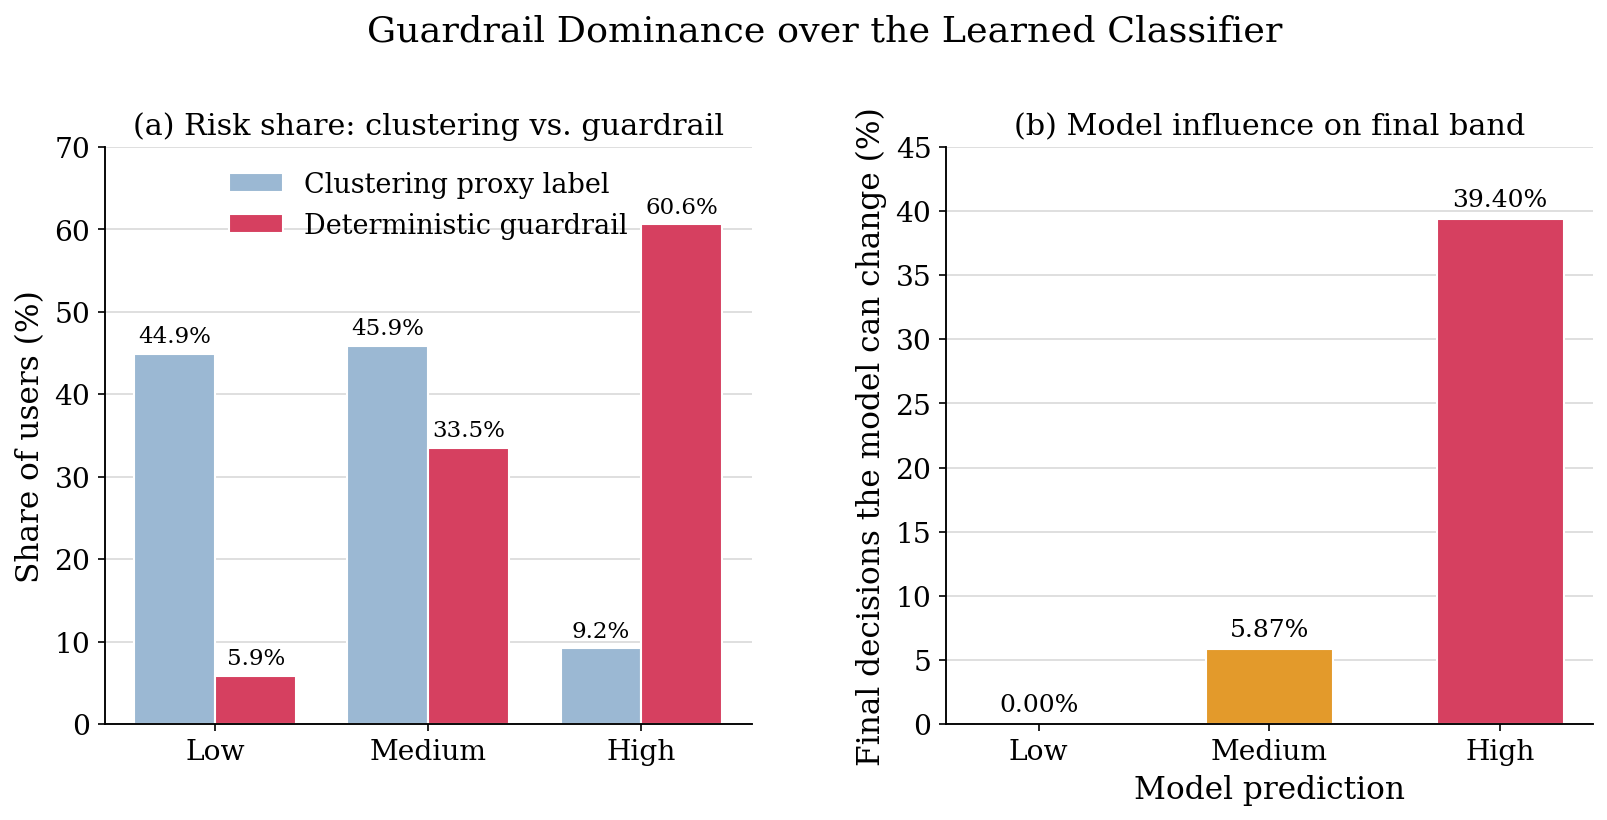
\includegraphics[width=0.9\linewidth]{fig_guardrail_dominance.png}
\caption{Guardrail dominance. (a) Risk share under clustering alone versus the guardrail
alone; the guardrail escalates 60.6\% of users to High risk. (b) Share of cases in which
the model prediction can still change the final band, by predicted class.}
\label{fig:guardrail}
\end{figure}

\subsection{Portfolio Simulation}\label{subsec:portfolio-sim}
\textbf{\textit{Simulation result.}} Under the deterministic twelve-month projection with
fixed monthly returns, the corrected return on investment is 25.72\% for the Low-risk
allocation, 15.40\% for Medium, and 2.43\% for High, against a USDC-only baseline of
2.43\% (Table~\ref{tab:roi}, Fig.~\ref{fig:roi}). Maximum drawdowns are $-3.79\%$,
$-2.08\%$, and 0.00\% respectively. The High allocation and the baseline coincide exactly
because a High-risk user is placed entirely in USDC.

\begin{table}[t]
\centering
\caption{Original versus corrected twelve-month ROI by risk band}
\label{tab:roi}
\begin{tabularx}{\linewidth}{@{}l C C C C@{}}
\toprule
Risk band & BTC/ETH/USDC & Original ROI & Corrected ROI & Max drawdown \\
\midrule
Low & 35 / 35 / 30 & 20.18\% & 25.72\% & $-3.79\%$ \\
Medium & 20 / 20 / 60 & 12.34\% & 15.40\% & $-2.08\%$ \\
High & 0 / 0 / 100 & 2.22\% & 2.43\% & 0.00\% \\
\midrule
Baseline (USDC) & 0 / 0 / 100 & --- & 2.43\% & 0.00\% \\
\bottomrule
\end{tabularx}
\end{table}

\begin{figure}[t]
\centering
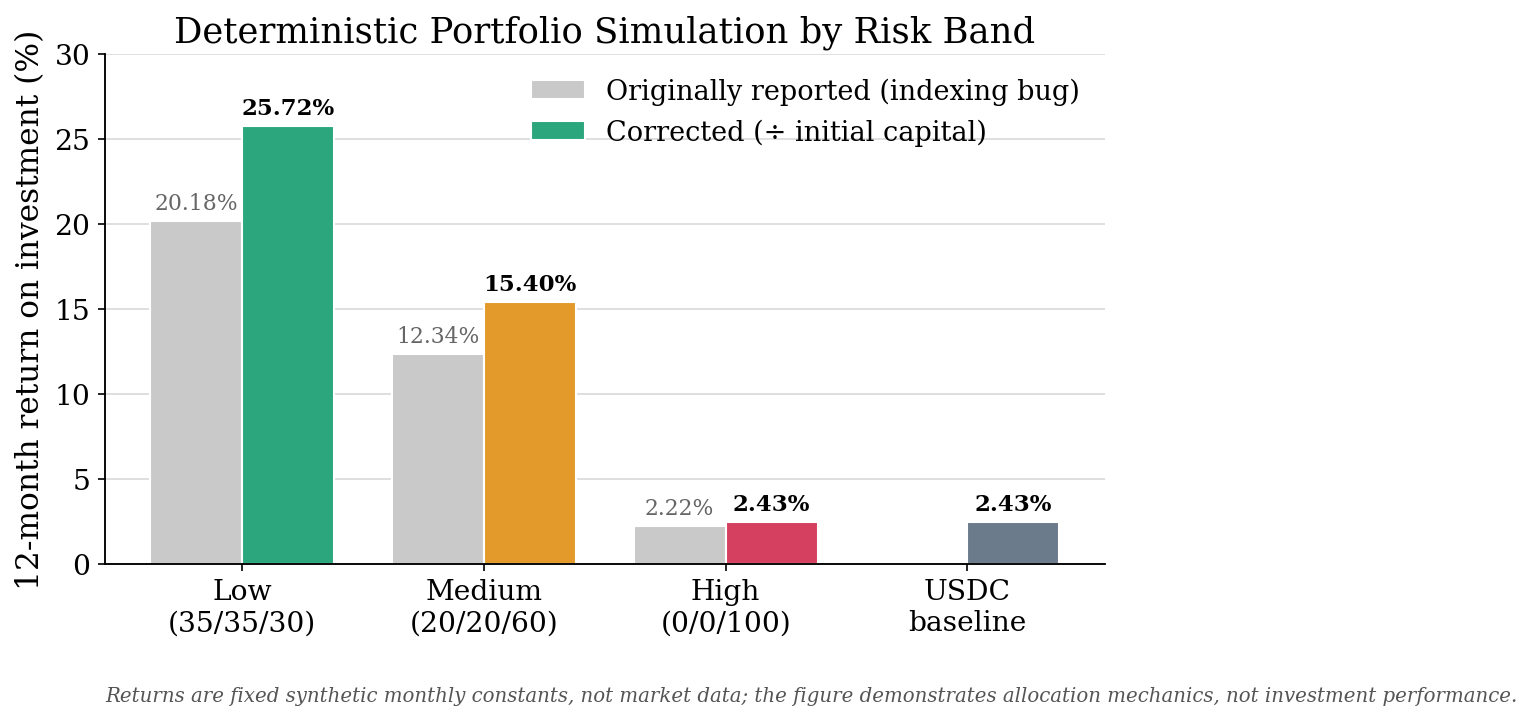
\includegraphics[width=0.72\linewidth]{fig_portfolio_roi.png}
\caption{Deterministic twelve-month simulated ROI by risk band: originally reported values
(inflated by the backtester indexing error) versus corrected values, against the USDC-only
baseline. The returns are fixed synthetic constants, so the figure demonstrates allocation
mechanics rather than market performance.}
\label{fig:roi}
\end{figure}

Two cautions attach. First, these are the corrected values: the originally reported ROIs
were inflated by an off-by-one normalization in the backtester. Second, and more
fundamentally, the returns are generated from fixed, hardcoded monthly constants rather
than live or historical market data, so they demonstrate the mechanics of the allocation
policy---higher assessed risk yields a more conservative, lower-variance allocation---but
are not evidence of real-world investment performance. They are best read as an internal
consistency check on the allocation logic.

\subsection{Auditability}\label{subsec:audit}
\textbf{\textit{Theoretical property.}} Every recommendation is hashed with SHA-256 over a
canonicalized payload and stored with a unique transaction identifier, and a verification
routine re-hashes a stored record to detect alteration. Tamper-evidence here is a property
of the cryptographic construction rather than a measured outcome: any change to a logged
payload changes its digest and is detectable on verification. The mechanism is exercised
against an in-memory simulated ledger, not a deployed blockchain, so it demonstrates the
auditability pattern rather than production-grade distributed immutability.

% =====================  SECTION V  =====================
\section{Discussion}\label{sec:discussion}

\subsection{Interpretation of Findings}\label{subsec:interpretation}
The results support a nuanced reading of the system. The integration objective is met: a
single user's raw inputs flow, without manual intervention, into an explained,
risk-aligned, and independently verifiable recommendation, and the safety properties hold
by construction rather than by training. What the evaluation also shows is that the
headline classification accuracy is the wrong summary of how the system behaves. The
deterministic guardrail escalates 60.6\% of users to High risk on cash-flow grounds and is
the binding signal for the majority, so the learned model is decisive for only a minority
of users; its 91.0\% accuracy is a real property of one component, measured on held-out
data, but says little about end-to-end decision quality. The comparative and statistical
results reinforce this modest reading: the MLP is statistically indistinguishable from
logistic regression, which in fact edges it on both area-under-curve metrics, so a neural
model is not shown to be necessary. These are not incidental caveats---they are the central
empirical content of the evaluation, and reporting them is part of the contribution.

\subsection{Engineering versus Research Contribution}\label{subsec:contribution-framing}
Separating the two kinds of contribution is what keeps the claims honest. The engineering
contribution is real and is the substance of the work: an integrated pipeline that unifies
feature engineering, unsupervised proxy labeling, a leakage-aware classifier, a
conservative guardrail, most-cautious reconciliation, model-adaptive explanation,
risk-aligned allocation, deterministic simulation, and a hashed, verifiable audit log in
one inspectable system with an explicit feature contract and a safety layer that cannot
lower risk. That combination is exactly what the reviewed literature treats as missing. The
research contribution is stated more modestly: the individual techniques are standard, and
the results do not establish that any is novel or that the learned model beats a simple
baseline. What the work contributes on the research side is methodological---a
demonstration that an integrated financial-recommendation pipeline can be held to an honest
evidential standard in which leakage is measured, guardrail dominance is quantified, and a
model-selection result that fails significance is reported rather than dropped. Ordinary
component integration is claimed nowhere as novel, and no claim is made of validation
against real financial outcomes.

\subsection{Limitations}\label{subsec:limitations}
The critical review surfaced seven limitations, stated here plainly with their severity in
Table~\ref{tab:limitations}. Three are of high severity. Guardrail dominance means the
accuracy figure does not describe end-to-end behavior. Arithmetic label leakage means that,
although the three ratios are withheld from the classifier at the column level, surplus and
expense ratio are deterministic functions of the raw inputs and are therefore recoverable,
making the classification task easier than one with independent labels; the strong
surplus--expense-ratio correlation in Fig.~\ref{fig:corr} is the empirical footprint of
this dependency. Most fundamentally, the labels are proxies produced by clustering, not
recorded default or loss outcomes, so no real-world predictive validity is established. The
medium-severity items are the statistically unjustified selection of the MLP over logistic
regression, the corrected backtest indexing error (which even corrected rests on fixed
synthetic returns), and entity leakage from a row-level split over data with only 944
unique users among 3,000 rows. Finally, at low-to-medium severity, part of the source tree
is a not-yet-extracted presentation layer, the ledger is an in-memory simulation rather
than a deployed chain, and the explainer is occlusion-based rather than SHAP or a
partial-derivative method.

\begin{table}[t]
\centering
\caption{Summary of limitations and their effect on claims}
\label{tab:limitations}
\setlength{\tabcolsep}{4pt}
\begin{tabularx}{\linewidth}{@{}p{3.2cm} >{\centering\arraybackslash}p{1.4cm} L@{}}
\toprule
Limitation & Severity & Effect on claims \\
\midrule
Guardrail dominance & High & Accuracy does not describe end-to-end decision quality. \\
Arithmetic label leakage & High & Classification easier than with independent labels. \\
Proxy labels, no ground truth & High & No real-world predictive validity established. \\
Non-significant model selection & Medium & MLP not statistically better than logistic regression. \\
Backtest indexing error & Medium & Original ROIs inflated; corrected values used. \\
Entity leakage in split & Medium & Generalization may be overstated. \\
Fa\c{c}ade layer / simulated ledger & Low--Med & Prototype-stage engineering, not production. \\
\bottomrule
\end{tabularx}
\end{table}

\subsection{Threats to Validity}\label{subsec:threats}
The limitations map onto the standard categories of validity as follows, so that a reader
can locate each concern precisely.

\begin{itemize}
\item[\textbf{Internal.}] The arithmetic recoverability of two clustering features from the
  classifier inputs, and the row-level split over repeated identifiers, both create paths
  by which apparent performance can be inflated relative to a genuinely independent
  prediction task.
\item[\textbf{Construct.}] The target is a clustering-derived proxy for risk, not a
  recorded financial outcome; the twelve-month ROI is computed from fixed constants rather
  than market data. Both measure the intended construct only indirectly.
\item[\textbf{External.}] The data are synthetic and single-source, and the returns are
  hardcoded, so results should not be extrapolated to real users or markets without
  revalidation on recorded data.
\item[\textbf{Conclusion.}] The small High-risk support (62 holdout cases) widens the
  interval on its per-class F1, and the McNemar tests are underpowered to detect small
  differences; the non-significant results are therefore reported as an absence of
  demonstrated superiority rather than proof of equivalence.
\end{itemize}

\subsection{Research Questions and Objective Fulfillment}\label{subsec:rq-fulfillment}
Table~\ref{tab:rqmap} closes the loop between the six research questions of
Section~\ref{subsec:rqs} and the evidence gathered in Section~\ref{sec:results}, assigning
each an explicit status of Supported, Partially supported, or Not demonstrated together
with the method and result that justify it. The verdicts are deliberately mixed. Three
questions are fully supported: the clustering yields coherent, monotonically ordered proxy
bands (RQ2), the reconciliation enforces an over-warn failure mode by construction (RQ4),
and the allocation-and-audit path produces tamper-evident, re-verifiable records (RQ6). The
remaining three are only partially supported, and are labelled so on purpose---risk can be
assessed from the withheld-ratio inputs, but column-level separation does not remove the
residual arithmetic leakage (RQ1); the classifier reproduces the labels with high accuracy,
yet a neural model is not shown to be warranted over logistic regression (RQ3); and the
explanation mechanism returns per-decision attributions without retraining, but only its
MLP branch is exercised in deployment (RQ5).

\begin{table*}[t]
\centering
\caption{Mapping of research questions to methods, evidence, and status}
\label{tab:rqmap}
\footnotesize
\setlength{\tabcolsep}{5pt}
\renewcommand{\arraystretch}{1.15}
\begin{tabularx}{\textwidth}{@{}>{\centering\arraybackslash}p{0.8cm} L L L >{\raggedright\arraybackslash}p{1.9cm}@{}}
\toprule
RQ & Research question / objective & Method / experiment & Evidence / result & Status \\
\midrule
RQ1 & Assess risk from raw, deployable inputs while withholding the label-defining ratios,
so leakage is explicit. &
Feature contract partitioning $F_{\text{cls}}$ and $F_{\text{clu}}$
(Eq.~\ref{eq:contract}) with a validation abort; residual-leakage analysis
(Sec.~\ref{subsec:contract},~\ref{subsec:limitations}). &
Classifier uses five raw inputs only; column separation is enforced, but surplus and
expense ratio stay arithmetically recoverable, so leakage is measured and disclosed rather
than removed. &
Partially supported \\
\addlinespace
RQ2 & Do interpretable-ratio clusters form coherent, monotonically ordered Low/Medium/High
proxy bands? &
K-means ($k = 3$) on standardized ratios; silhouette, Calinski--Harabasz,
Davies--Bouldin, and ARI stability; cluster profiling (Table~\ref{tab:cluster}). &
Silhouette 0.370 and ARI $0.868 \pm 0.064$; mean surplus falls and mean expense ratio
rises monotonically from Low to High (Table~\ref{tab:cluster}). &
Supported \\
\addlinespace
RQ3 & Can a classifier reproduce the proxy labels from raw inputs with useful accuracy, and
is a neural model warranted over simpler baselines? &
MLP versus logistic regression, random forest, and decision tree; McNemar tests; five-fold
CV; bootstrap CIs (Tables~\ref{tab:perclass}--\ref{tab:stats}). &
91.0\% accuracy and 0.881 macro-F1, but the MLP is not significantly better than logistic
regression ($p = 0.100$) or random forest ($p = 0.176$), which even edge it on AUC. &
Partially supported \\
\addlinespace
RQ4 & Reconcile the learned, unsupervised, and rule-based signals so the failure mode is to
over-warn. &
Escalate-only guardrail (Eq.~\ref{eq:guardrail}) and most-cautious rule
$y^{*} = \max(m, g, k)$ (Eq.~\ref{eq:reconcile}); guardrail-dominance measurement
(Sec.~\ref{subsec:guardrail-dom}). &
Reconciliation cannot lower risk by construction; the guardrail is $\geq$ the cluster
signal for 100\% of users and escalates 60.6\% to High risk. &
Supported \\
\addlinespace
RQ5 & Provide per-decision, input-level attributions across model types without retraining.
&
Model-adaptive occlusion sensitivity (Eq.~\ref{eq:occlusion}): mean-imputation for the MLP,
signed coefficients for linear models, impurity for trees. &
Yields per-input influence scores for the deployed MLP without retraining; the other
branches exist by construction, but only the MLP branch is exercised. &
Partially supported \\
\addlinespace
RQ6 & Map the reconciled band to a risk-aligned crypto allocation and log a tamper-evident,
verifiable record. &
Deterministic band$\rightarrow$(BTC, ETH, USDC) map (Eq.~\ref{eq:alloc}); SHA-256 hashing
of a canonical payload with re-hash verification (Eq.~\ref{eq:hash}). &
Allocation is deterministic and risk-monotone; any change to a logged payload changes its
digest and is detected---though against an in-memory simulated ledger, not a live chain. &
Supported \\
\bottomrule
\end{tabularx}
\par\vspace{3pt}
{\footnotesize\itshape\raggedright The three `supported' verdicts rest on properties that
hold by construction (RQ4, RQ6) or on direct metric evidence (RQ2); the three `partially
supported' verdicts mark exactly where an honest reading stops short---residual leakage, an
unjustified neural model, and a single exercised explanation branch. No verdict claims
validation against real financial outcomes, which remains outside the scope of this
proxy-labelled study.\par}
\end{table*}

% =====================  SECTION VI  =====================
\section{Conclusion and Future Work}\label{sec:conclusion}

\subsection{Conclusion}\label{subsec:conclusion}
This paper set out to build an integrated, explainable, and independently verifiable
decision-support pipeline that carries a single user's raw financial inputs through risk
assessment, safety enforcement, explanation, portfolio allocation, and tamper-evident
logging---a combination the reviewed literature treats as five largely separate problems.
The pipeline delivers that integration end to end: it engineers three interpretable ratios
from five raw inputs, derives Low, Medium, and High risk segments by clustering (silhouette
0.370, stable at an adjusted Rand index of 0.868), trains a leakage-aware MLP that
reproduces the risk band at 91.0\% accuracy and 0.881 macro-F1, routes every prediction
through a conservative guardrail that can only escalate risk, explains each decision with a
model-adaptive feature-impact method, maps the reconciled band to a risk-aligned
BTC/ETH/USDC allocation, and records a SHA-256-hashed, verifiable receipt for every
recommendation.

Equally central to the conclusion is what the work does not claim. The evaluation
establishes that the conservative guardrail, not the learned model, determines most final
recommendations; that the proxy labels are arithmetically entangled with the classifier
inputs; that the MLP is not statistically better than logistic regression; and that the
portfolio simulation rests on fixed synthetic returns. The contribution is therefore an
engineering one---a coherent, inspectable integration of standard techniques with an
explicit feature contract and a safety-first reconciliation---reported against an honest
evidential standard rather than an inflated one. In answering its six research questions,
the work shows that such a pipeline can be built and made transparent, while remaining
candid that demonstrating real-world predictive validity lies outside its present scope.

\subsection{Future Work}\label{subsec:future-work}
The limitations map directly onto a program of future work, ordered by how much each would
strengthen the evidential standing of the system:

\begin{itemize}
\item[\textbf{1)}] Replace the clustering-derived proxy labels with recorded default or
  loss outcomes, so the classifier predicts a ground-truth target rather than a clustering
  artifact \cite{ref18,ref19}.
\item[\textbf{2)}] Adopt entity-level (grouped) splitting by identifier to remove the
  entity-leakage concern and yield a trustworthy generalization estimate.
\item[\textbf{3)}] Break the arithmetic label dependency by constructing labels from
  information not fully recoverable from the classifier inputs, or by explicitly modeling
  that dependency.
\item[\textbf{4)}] Rebalance the guardrail and the model---including resolving the 60/75
  medium-threshold inconsistency---so the learned component contributes to more decisions.
\item[\textbf{5)}] Strengthen the explanation layer by adopting SHAP or a partial-derivative
  sensitivity method and combining attributions, as the benchmark literature recommends
  \cite{ref10,ref21}.
\item[\textbf{6)}] Integrate historical or live market and DeFi data, modeling the
  liquidation and stablecoin-instability risks documented in the literature, to turn the
  deterministic projection into a genuine backtest \cite{ref5,ref6}.
\item[\textbf{7)}] Deploy a real audit ledger via a smart contract, with attention to
  storage, throughput, and oracle-trust costs, to make the auditability claim
  production-grade \cite{ref13,ref14,ref15,ref22}.
\item[\textbf{8)}] Move toward dynamic, causal allocation---reinforcement-learning
  rebalancing or an explainable optimizer---framed with the causal-inference caution raised
  for financial planning \cite{ref4,ref8,ref12}.
\end{itemize}

Taken together, these directions would progressively convert the present prototype---an
honest demonstration of integration---into a system whose predictive and financial claims
could be defended on external evidence. That progression, rather than any single algorithmic
advance, is the path these findings point toward.


% ---- References -------------------------------------------------------------
\bibliographystyle{IEEEtran}
\bibliography{references}

\end{document}
